\documentclass{article}
\usepackage{arxiv}
\usepackage[utf8]{inputenc}
\usepackage[T1]{fontenc}    % use 8-bit T1 fonts
\usepackage{hyperref}       % hyperlinks
\usepackage{url}            % simple URL typesetting
\usepackage{booktabs}       % professional-quality tables
\usepackage{amsfonts}       % blackboard math symbols
\usepackage{amsmath}
\usepackage{nicefrac}       % compact symbols for 1/2, etc.
\usepackage{microtype}      % microtypography
\usepackage{lipsum}
\usepackage{graphicx}
\usepackage{float}
\usepackage{subcaption}
\usepackage[ruled,vlined]{algorithm2e}
\usepackage{cleveref}

\usepackage{todonotes}
\newcommand{\comment}[1]{\todo[color=orange!40, inline]{\footnotesize{#1}}}
\newcommand{\kleidi}[1]{\todo[color=green!40, inline]{\footnotesize{Kleidi: #1}}}
\newcommand{\henrique}[1]{\todo[color=blue!40, inline]{\footnotesize{Henrique: #1}}}
\newcommand{\yves}[1]{\todo[color=yellow!40, inline]{\footnotesize{Yves: #1}}}
\newcommand{\serge}[1]{\todo[color=purple!40, inline]{\footnotesize{Serge: #1}}}


\title{Ranking the output of static analysis}
\author{Kleidi Ismailaj \\ \\ \href{mailto:kleidi.ismailaj@student.uantwerpen.be}
{\textit{kleidi.ismailaj@student.uantwerpen.be}}}
\date{\today}

\begin{document}

\maketitle
\newpage
\tableofcontents
\newpage

\section{Abstract}
Previous research has estimated the number of false positive static analysis alerts to be as high as 70\% (\textbf{TO DO: CITE}). Research has also shown that developers loose trust and ignore such tools when the number of false positive (or unimportant) alerts is high. Given that static analysis is still helpful in promoting cleaner code, different aspects from the history of the codebase can be exploited to improve the relevance of the output. If the output is matched to what the developer finds important or what has been proven to be helpful in the past, this will lead to a better acceptance and wider usage of such tools.

% I try to have four sentences in my abstract. The first states the problem. The second states why the problem is a problem. The third is my startling sentence. The fourth states the implication of my startling sentence. An abstract for this paper done in this style would be:

% The rejection rate for OOPSLA papers in near 90\%. Most papers are rejected not because of a lack of good ideas, but because they are poorly structured. Following four simple steps in writing a paper will dramatically increase your chances of acceptance. If everyone followed these steps, the amount of communication in the object community would increase, improving the rate of progress. 

\section{Introduction}
% This is a general introduction to what the thesis is all about -- it is not just a description of the contents of each section. Briefly summarize the question (you will be stating the question in detail later), some of the reasons why it is a worthwhile question, and perhaps give an overview of your main results. This is a birds-eye view of the answers to the main questions answered in the thesis (see above). 

% +Positive aspects of SA and usages (google, fb etc...), their need (huge amounts of code), etc...\\

The amount of code that is being produced is increasing with time. That brings multiple challenges in the software engineering landscape, one of which is assuring adequate code quality. In this context, automatic approaches such as static analysis can be really useful and time saving in detecting and preventing potential bugs. Its usefulness has been acknowledged also by big tech companies, such as Google with its Tricorder architecture (\cite{sa_google}) or Facebook with its Infer static analyzer.
Another reason to adopt SA techniques, is that the cost of repairing a defect is much lower when that defect is found early in the development cycle (generally accepted principle).

Even though it is a promising technique, in practice static SA results are far from perfect. Since the software under analysis is not executed, static analysis tools must speculate on what the actual program behavior will be, thus mistakes are inevitable. Heuristics or approximations are commonly used to determine properties for a given code construct, which may lead to inaccurate assumptions. A tool can also deliberately introduce approximations for scalability or speed, potentially resulting in an outbreak of errors.

Given the ever increasing amount of code and the tendency of SA tools to over-estimate possible faulty program behaviours, there is a need to improve the output of these tools. The above problem can be addressed either by increasing the precision of the analysis (and thus decrease the efficiency) or by post-processing the alarms effectively after they are generated, according to specific criteria.
The classic approach most tools use for prioritizing and filtering results is to statically classify the results based on severity levels. They are oblivious of the actual code that is being analyzed and of the location or frequency of a given defect. Furthermore, it has been shown that if developers lose trust in the beginning, they then tend to ignore the output of these tools altogether (\textbf{TO DO: CITE}).

Different approaches have been proposed to improve the output of SA tools. Optimally, the initial error reports should be those most likely to be real errors. Alerts can be strategically prioritized for examination, by tracking warnings through a series of software versions, revealing which SA rules are more important and which parts of the software are more problematic. 
% Furthermore, alerts can be grouped/clustered in basis of their similarity, so that users can check only a few and then can easily determine if the rest of the errors are also worth inspecting.\\
An understanding of how developers react on these alerts can help improve the utility of these tools. Alerts can be divided into two categories: actionable alerts (AA) to define a SA alert that the programmer would act on to resolve and unactionable alerts (UA) to define a SA alert that the programmer would not act on to resolve (\textbf{TO DO: CITE}). An unactionable alert may be: a trivial concern to fix, less likely to manifest at runtime, or incorrectly identified due to the limitations of the tool. We want thus to prioritize the AAs and hide the UAs.

Another approach is to prioritize alerts that in the past have pointed at bugs (\textbf{TO DO: CITE}). By tracking back the bugs up to a certain revision in the past, we can collect code lines that were changed during bug(\textbf{TO DO: CITE}) fixes. Subsequently, we can pinpoint which alerts warned about those specific parts of code and prioritize accordingly.

Given that for a relatively large project, the number of SA alerts can be prohibitive, the ultimate goal is to maximize the utility of time spent analyzing these alerts. Ranking schemes do not reduce alert investigation burdens if the aim is to check them all. Instead, they solve the problem by showing alerts that are most likely to be real/useful, so that developers can spend time by inspecting the most important ones.
% , but the number of alarms to investigate is not reduced with ranking.

Different approaches have been proposed in the literature but few have tried to do a comparison in terms of the utility of each method. Comparison is done among open source Java software and has the following problems... (\textbf{TO DO: FILL IN}). Also, these methods can be combined with the aim of achieving better results. It is important to do so because different techniques can be better suited to different types of alerts or can compensate for each others weaknesses.

% (depending also on the information that can be extracted from the source code).

% -what is this student's research question?
% -is it a good question? (has it been answered before? is it a useful question to work on?) 

Given an industrial code base, where SA tools have been abandoned because of the large amount of false positives, the goal of this thesis is to test the feasibility of successfully applying these ranking approaches even in a context with limited amount of data.

% The research questions can be formulated as follows:
% \begin{itemize}
%     \item R0: Can we apply SA ranking techniques in an industrial environment with limited amount of data (abandoned because of high false positives)?
%     \item R1: Given a highly imbalances dataset, what are the best performing dataset balancing techniques?
%     \item R2: Can we process the collected data to remove faulty examples (CLNI?) (project specific bugs?) (fix the data not the algorithms)
%     \item R3: Can we combine SA ranking techniques to achieve better results?
% \end{itemize}

% In this thesis, a comparison of different SA processing approaches is performed in an industrial codebase. Also, the utility of combining different methods is explored.

The rest of this thesis will be structured in the following sections... (\textbf{TODO})

% \textbf{TO DO: duality, actionable alert and bug predicition alerts}

% \textbf{TO DO: add class/method to each alert}

% \textbf{TO DO: Collect line from alert}

% \textbf{TO DO: Try clang automatic fixes}


% Arguments/information gotten from papers that can be used for the thesis introduction.
% \begin{itemize}
%     \item Why the false positives?
%     \begin{itemize}
%         \item Inevitable mistakes (SA has to make a trade-off with efficiency).
%         \item Static analyzers commonly use heuristics or approximations to determine properties for a given code construct, which frequently induces them to make inaccurate assumptions regarding the behavior of the program under evaluation.
%         \item A tool may deliberately introduce approximations for scalability or speed or to check richer properties than is generally possible, potentially resulting in an outbreak of errors. By ranking the results the invalid errors can be relegated below true errors.
%         \item Because the software under analysis is not executed, static analysis tools must speculate on what the actual program behavior will be. They often over-estimate possible program behaviors, leading to spurious warnings (“false positives”) that do not correspond to true defects.
%     \end{itemize}

%     \item Why its important to rank warnings (show the most relevant subset) or reduce false positive?
%     \begin{itemize}
%         \item The classic approach most automated code inspection tools use for prioritizing and filtering results is to classify the results based on severity levels. Such levels are (statically) associated with the type of defects detected; they are oblivious of the actual code that is being analyzed and of the location or frequency of a given defect.
%         \item Empirically, all tools that effectively find errors have false positive rates that can easily reach 30–100\%.
%         \item In general, there are roughly 40 warnings for every thousand lines of code [11]. This overload of warnings is a prime reason for developers to avoid using ASATs [12]. (\cite{analysis_sa_usage})
%         \item False reports can easily render tools useless by hiding real errors amidst the false, and by potentially causing the tool to be discarded as irrelevant.
%         \item Warnings are not always acted on by developers even if they reveal true defects. Reasons for defects being ignored include warnings implicating obsolete code, “trivial” defects with no impact on the user, and real defects requiring significant effort to fix with little perceived benefit.
%         \item The effort required to manually audit all alerts and repair all confirmed code flaws is often too much for a project’s budget and schedule.
%     \end{itemize}

%     \item How to improve?
%     \begin{itemize}
%         \item An understanding of how developers react on the alerts detected by SA tools can help improve the utility of these tools and determine future research directions.
%         \item The initial few error reports should be those most likely to be real errors so that the user can easily see if the rest of the errors are worth inspecting (otherwise users tend to discard the tool).
%         \item \textbf{Strategically prioritizing} alerts for examination.
%         \item Results indicate that using several ASATs has benefits over using just a single ASAT. (\cite{analysis_sa_usage})
%         \item Tracking warnings through a series of software versions reveals where potential defects are commonly introduced and addressed, and how long they persist; thus exposing interesting trends and patterns. This helps in determining which SA rules are important for a software system and helps select a minimum set of rules that must be enabled.
%     \end{itemize}

%     \item We use the term actionable alert (AA) to define a SA alert that the programmer would act on to resolve and unactionable alert (UA) to define a SA alert that the programmer would not act on to resolve.
    
%     \item Only show \textbf{actionable alerts}.
%     An unactionable alert may be one of the following: 1) a trivial concern to fix, 2) less likely to manifest in runtime environment; or 3) incorrectly identified due to the limitations of the tool.
    
    
%     % \item It is generally accepted that the cost of repairing a defect is much lower when that defect is found early in the development cycle.
    
%     % \item The above problem of alarms and associated cost can be addressed either by improving precision of the analysis or by postprocessing the alarms effectively after they are generated.
    
%     % \item Note that the above described handling of alarms does not consider reducing the number of alarms \textbf{by making underlined static analysis more precise}. That is, it excludes the option of improving precision of analyses, like value analysis and pointer analysis, implemented in the static analysis tools.
    
%     % \item However, even when tools focus on uncovering the same defect type, the variance in defects found is still very large [6],[13]–[15]. These results indicate that using several ASATs has benefits over using just a single ASAT. (\cite{analysis_sa_usage})
    
%     \item ranking schemes do not reduce alarm-investigation burdens - alleviate the false alarm problem by showing alarms that are most likely to be real errors over those that are least likely. However, the number of alarms to investigate is not reduced with ranking.
    
% \end{itemize}

\newpage

\section{Problem statement}
\henrique{To me, a problem statement section should appear as earlier as possible in the thesis. It can even be a subsection of the introduction. }
% Research Question or Problem Statement

% Engineering theses tend to refer to a "problem" to be solved where other disciplines talk in terms of a "question" to be answered. In either case, this section has three main parts:

% 1. a concise statement of the question that your thesis tackles
% 2. justification, by direct reference to the literature review, that your question is previously unanswered
% 3. discussion of why it is worthwhile to answer this question.

% Item 2 above is where you analyze the information which you presented in Section 3. For example, maybe your problem is to "develop a Zylon algorithm capable of handling very large scale problems in reasonable time" (you would further describe what you mean by "large scale" and "reasonable time" in the problem statement). Now in your analysis of the state of the art you would show how each class of current approaches fails (i.e. can handle only small problems, or takes too much time). In the last part of this section you would explain why having a large-scale fast Zylon algorithm is useful; e.g., by describing applications where it can be used.

% Since this is one of the sections that the readers are definitely looking for, highlight it by using the word "problem" or "question" in the title: e.g. "Research Question" or "Problem Statement", or maybe something more specific such as "The Large-Scale Zylon Algorithm Problem." 

Improving the output of static analysis is dependent on a particular codebase and the people who produce it. Different organizations can have different priorities and expectations on code quality. Also developers or teams might be more interested on a particular subset of warnings (or the context on which the warnings appear).

Given an industrial codebase, the goal is to explore if these automatic techniques are useful, which produces the best results, and if an ensemble technique provides extra benefits. The starting point is the version control history of the project. By extracting information about the past versions, an attempt can be made to learn which SA alerts are more important and can be prioritized in the future. In contrast to open source project where you can test the approaches only on those project that have a sufficient amount of data, in an industrial codebase you have to make the most of the data you can extract. This thesis examines which ML techniques can be used to deal with highly imbalanced or noisy data.

Two main approaches are explored: detecting actionable alerts (alerts deemed useful by the developers) and alerts that aid in detecting bugs. These approaches are complementary because the sets of alerts are not necessarily equal, thus they are a good candidate for a combination.

The research questions can be formulated as follows:
\begin{itemize}
    \item R0: Can we apply SA ranking techniques in an industrial environment with limited amount of data (abandoned because of high false positives)?
    \item R1: Given a highly imbalanced and noisy dataset, what are the best performing dataset balancing techniques?
    % \item R2: Can we process the collected data to remove faulty examples (CLNI?) (project specific bugs?) (fix the data not the algorithms)
    \item R2: Can we combine SA ranking techniques to achieve better results?
\end{itemize}

This research is important because it quantitatively examines if the version history of a project combined with machine learning techniques can be used to effectively improve the output of SA tools. By doing so, we can examine the real utility of this approach in practice and identify which techniques are more effective. It is also relevant to see if these approaches produce meaningful results in the case of limited amount of data. We can observe the impact in performance by testing different ML techniques to reduce noise and balance the dataset (like under and oversampling). 

Based on the literature review, few papers make direct comparisons between different methods on a common experiment baseline (\textbf{TO DO: cite papers}). Also, they focus on open source Java systems with an adequate amount of data. One paper researches the impact of noisy data and proposes a solution (\textbf{TO DO: cite clni}). Regarding ensemble techniques, there have been approaches where multiple SA tools are combined, or where each alert types is handled by its own classifier. In contrast, we focus on C++ code and compare different preprocessing techniques. Also, we try an ensemble approach with two different methods of ranking SA alerts.

\section{Background}

\henrique{A Background section is not an Appendix. Specially for a thesis such as this, the main concepts you want to describe are important for a reader to better understand the techniques used.}

% What goes in the appendices? Any material which impedes the smooth development of your presentation, but which is important to justify the results of a thesis. Generally it is material that is of too nitty-gritty a level of detail for inclusion in the main body of the thesis, but which should be available for perusal by the examiners to convince them sufficiently. Examples include program listings, immense tables of data, lengthy mathematical proofs or derivations, etc. 

Possible concepts to explain/introduce in the thesis background section:
\begin{itemize}
    \item Bayesian networks
    \item ML algorithms
    % \item Logistic regression
    % \item Principal component analysis
    % \item Correlation methods
    \item Precision, recall, auc \henrique{We usually describe Precision, Recall and other metrics used in the Evaluation as a subsection inside the evaluation.}
    % \item Deep learning
    % \item Clang AST (if used)
\end{itemize}


\section{Literature review \label{literature}}

This section will consist of research papers focused on these main topics: 
\begin{itemize}
    \item \textit{Ranking static analysis alerts}: some of the most known (cited) approaches to rank alerts.
    \begin{itemize}
        \item Using a single SA tool
        \item Combining multiple tools
        \item Looking at survey papers that describe the state of the research and state of the art techniques.
        \item Comparative studies evaluating different methods.
    \end{itemize}
    \item \textit{Bug prediction}: Rank the alerts in problematic parts of code higher.
    \item Information on \textit{real world usage of SA tools}, problems and suggested solutions.
\end{itemize}

 \subsection{Dealing with False Positives}

 \subsubsection{Single Tool}

 Kremenek and Engler \cite{z-ranking} introduce \textit{Z-ranking}, a statistical model to rank the error reports of SA tools. They make a distinction between successful and failed checks (those that satisfy a checked property and those that violate it). The underlying observation is that the most reliable error reports are those that generated few failed checks and many successful checks, since the actual amount of bugs in code is relatively small. An explosion of failed checks is a likely indicator that something is going wrong with the analysis. Reports are sorted based on the calculated \textit{z-test} statistic (based on the relative frequency of successful and failed checks).

 The problem can be formally defined as a classification task. Let P be the population of all reports, both successful checks and failed checks, emitted by a program checker analysis tool. \textit{P} consists of two subpopulations: \textit{S}, the subpopulation of successful checks and \textit{E}, the subpopulation of failed checks (or error reports). The set of error reports \textit{E} can be further broken down into two subpopulations: \textit{B}, the population of true errors or bugs and \textit{F}, the population of false positives. The classification problem can then be restated as follows: given an error report $x \in E$, decide which of the two populations \textit{B} and \textit{F} it belongs to. That is based on the fact that \textit{B} and \textit{F} have different statistical characteristics. 

 Given a grouping operator \textit{G} that groups successful and failed checks together, we calculate the proportion of failed checks $G.\rho = \frac{G.successful}{G.failed}$. Populations are ranked both by the $\rho$ value and by the degree of confidence in its estimation. By treating these checks inside the groups as a sequence of binary trials (coin tosses). The probability $p_i$ of success will have to be approximated using the standard error. By using the \textit{z-test} statistic, which measures how far an observed value is from the real population, a value can be specified that produces a large positive \textit{z-score} when there are few errors and many successes, and a large negative \textit{z-score} when there are few successes and many errors.

 Given an estimated $p_i$ and a calculated \textit{SE}, we can chose $p_0$ to produce the effect mentioned above:
 $z=\frac{observed-expected}{SE}=\frac{p_i-p_0}{SE}=\frac{p_i-p_0}{\sqrt{\frac{p_0(1-p_0)}{n}}}$. The average population success rate can be chosen as a starting point for the value of $p_0$.

 According to their tests, \textit{Z-ranking} performed better than randomized ranking 98.5\% of the time. Moreover, within the first 10\% of reports inspected, \textit{Z-ranking} found 3-7 times more real bugs on average than found by randomized ranking.\\

 \begin{figure}[H]
     \begin{subfigure}{1\textwidth}
         \centering
         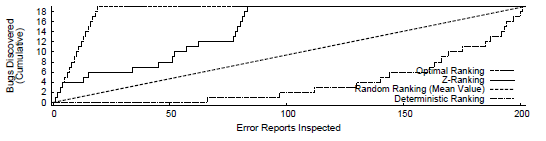
\includegraphics[scale=0.7]{./src/z_ranking_result_linux_intra.png}
         \caption{Intra-procedural check on Linux spin (lock)}
     \end{subfigure}\\
     \begin{subfigure}{1\textwidth}
         \centering
         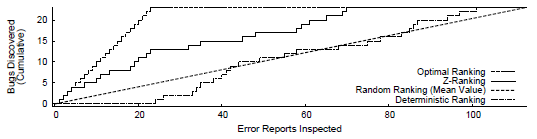
\includegraphics[scale=0.7]{./src/z_ranking_result_linux_inter.png}
         \caption{Inter-procedural check on Linux (free calls)}
     \end{subfigure}
 \end{figure}


 Kremenek et al. \cite{correlation_exploitation} introduce \textit{Feedback-Rank}, a dynamic ranking scheme that adapts as reports are inspected. By analyzing historical data, they observed that both bugs and false positives cluster by code locality. They present a probabilistic technique that exploits this correlation and also incorporates user feedback by reordering reports after each inspection. Since reports are correlated within a population (cluster), inspecting one of them yields information about the others. The ranking works by using a \textit{Bayesian Network} and exploiting two features, the number of populations (error messages grouped together) and the strength of correlation in each population. Furthermore, the strategy also continues improving with time, by taking into account the history of inspections.

 An intuitive explanation for the reason that reports cluster is given for both real and false positives. Regarding true positives, when developers do not know a rule, they will repeatedly violate it, so errors of the same type will correlate together. As for the false positives, there are three main causes: analysis mistakes of the tool (explosion of errors), rare coding idioms used by developers (which trigger the tools), incomplete rule specifications (a rule holds in most cases, but can be safely violated in others).

 To cluster the reports, code locality in different granularities is chosen: function, file and directory level. From the results in \cref{fr:lshape} it can be seen that very few populations contain a mix of bugs and false positives. \textit{Applicability} is defined as the ratio of non singleton clusters (which are bad for online ranking) to the total amount of clusters. The coarser the granularity the greater the applicability but also the smaller the correlation. \textit{Skew} is defined as the ratio of homogeneous clusters (all bugs or all false positives) to the total number of clusters. In this case, the more refined the granularity (function level), the higher the skew. Thus, a trade-off needs to be made between applicability and skew.

 To apply the algorithm a model is needed that produces the correlations among the reports. The reports are divided into two major regions, one that contains mostly true positive ($g_B$), and one that contains mostly false positives ($g_{FP}$) (see \cref{fr:partition}). A \textit{Bayesian Network} is used to calculate the probabilities of a cluster belonging to a certain region (regions are different for different granularities). The initial configuration can either be chosen by the user or learned from historical data. A simple model can be seen on \cref{fr:bayes}, where 3 reports depend on the probabilities of the parent function, file and directory clusters they belong to. Influence though, flows across both directions: if we inspect a report and know its value, the probabilities of the parents are re-calculated. Gives a training set, the conditional probability distributions of the network (along with the probabilities for the regions) can be learned using \textit{Expectation Maximization}. \textit{Belief Propagation} is used to update probabilities after each inspection and \textit{Information Gain} is used as a secondary factor to rank the reports. 

 Feedback-Rank represents a complementary approach to static ranking schemes (it can be combined with Z-Ranking for example) and can be trained with other forms of correlation instead of code locality. 

 According to their tests, \textit{Feedback-Rank} performed 2-8 times better than randomized ranking.\\

 \begin{figure}[H]
     \begin{subfigure}{1\textwidth}
         \centering
         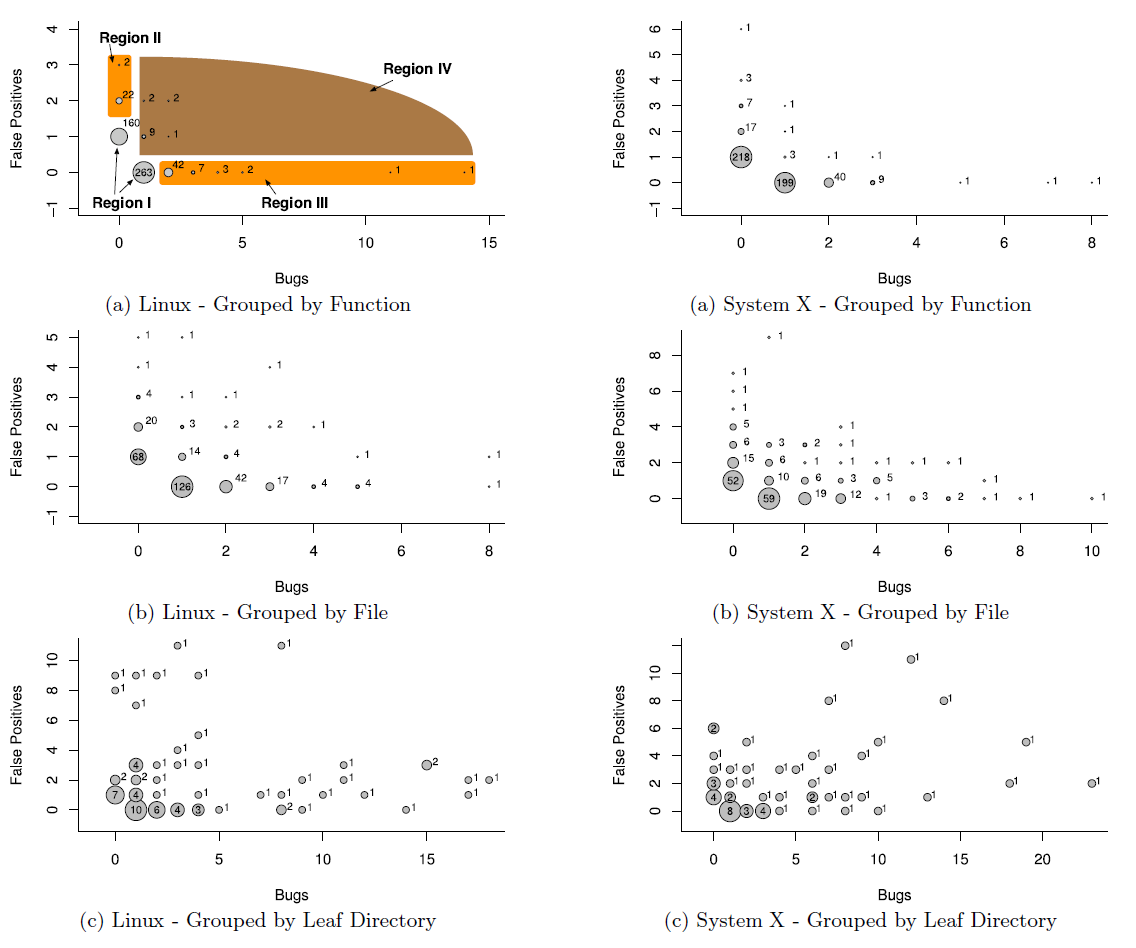
\includegraphics[scale=0.4]{./src/feedback_rank_l_shape.png}
         \caption{"L" shape of clustering}\label{fr:lshape}
     \end{subfigure}\\
     \begin{subfigure}{.5\textwidth}
         \centering
         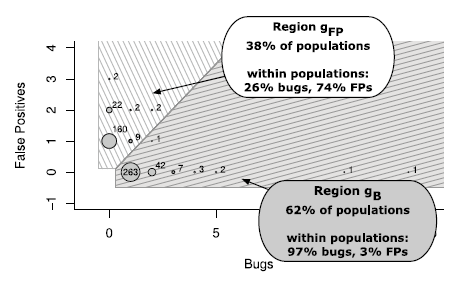
\includegraphics[scale=0.6]{./src/feedback_rank_partition.png}
         \caption{Populations divided into regions, mostly true or false positives}\label{fr:partition}
     \end{subfigure}%
     \begin{subfigure}{.7\textwidth}
         \centering
         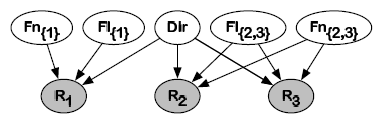
\includegraphics[scale=0.4]{./src/feedback_rank_bayes.png}
         \caption{Sample Bayesian network with 3 reports}\label{fr:bayes}
     \end{subfigure}
 \end{figure}


 Boogerd and Moonen \cite{static_profiling} present a technique, \textit{ELAN}, that prioritizes SA warnings by using the (predicted) likelihood that the execution reaches the location for which the warnings are reported. The execution likelihood is defined as the probability that a program point will be executed at least one in an arbitrary program run and is calculated statically. This computation is demand-driven, thus it is only performed for the locations associated with warning reports.

 The workflow (\cref{elan:workflow}) consists of normalizing the results of SA tools (to a specific format), creating system dependency graphs, calculating for every warning the likelihood of execution, ordering the results using the execution probability and possibly other external techniques (like Z-Ranking). 

 Likelihood analysis is based on system dependency graphs, which tie all program dependency graphs (function level) together by modelling the inter-procedural control dependencies. Their approach only considers control flow and ignore dataflow information. In order to avoid traversing all the SDG, \textit{program slicing} is used on control points. Other than the basic algorithm, they also introduce branch prediction heuristics, which do not excessively impact performance.

 Experiments show that predicted execution likelihoods correlate with data extracted from dynamic profiling. One problem though, is that when for example 30\% of all code is always executed, then the ranking of those warnings that belong to that piece of code, cannot be distinguished.

 \begin{figure}[H]
     \centering
     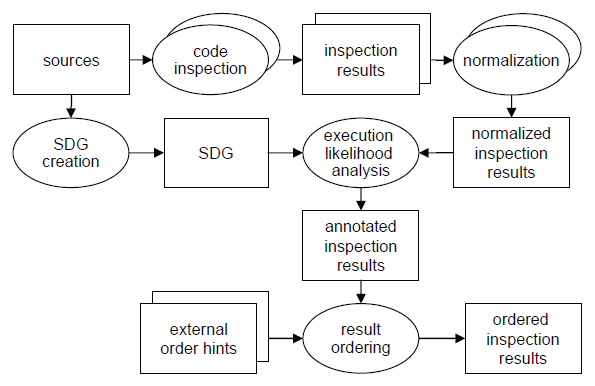
\includegraphics[scale=0.4]{./src/elan_workflow.png}
     \caption{Workflow for the ELAN tool}\label{elan:workflow}
 \end{figure}


 Kim and Ernst \cite{which_warnings} propose a history-based warning prioritization (HWP) algorithm which works by mining fix-changes in the VCS. It is based in the intuition that if a warning is removed by a fix, then probably that warning was important. On the other hand, if a warning instance is not removed for a long time, then warnings of
 that category may be neglectable, since the problem was not noticed or was not considered worth fixing. They measured the tool warning prioritization (TWP) on three different systems and found a precision of 3\%, 12\% and 8\%.  

 They set a weight to each warning category to represents its importance. The weight will be proportional to the number of warnings eliminated by changes (where fix-changes have the biggest weight, \cref{which_warnings:weights}). Selecting the top weighted warnings improves precision up to 17\%, 25\%, and 67\% respectively. Precision is calculated as $precision = \frac{number\:of \:warnings\:on\:bug\:related\:lines}{total\:number\:of\:warnings}$.
 By looking at the fix-changes and corresponding affected lines, by starting at the last revision, they can mark the bug-related lines, up to the first revision when they appeared (\cref{which_warnings:marking}). Ranking is category-based, so only the categories of warnings are considered and there is no distinction between the warnings inside each category. The algorithm works well if the categories are fine grained and internally homogeneous.

 They measure precision by training the weights in the first half of the version history, and testing them on the other half. The HWP outperforms TWP for all three systems (\cref{which_warnings:results}).

 \begin{figure}[H]
     \begin{subfigure}{0.6\textwidth}
         \begin{subfigure}{.5\textwidth}
             \centering
             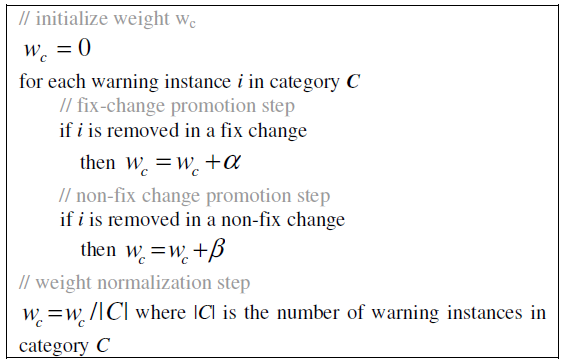
\includegraphics[scale=0.45]{./src/which_warnings_weights.png}
             \caption{Precision results at line-level}\label{which_warnings:weights}
         \end{subfigure}\\
         \begin{subfigure}{.5\textwidth}
         \centering
         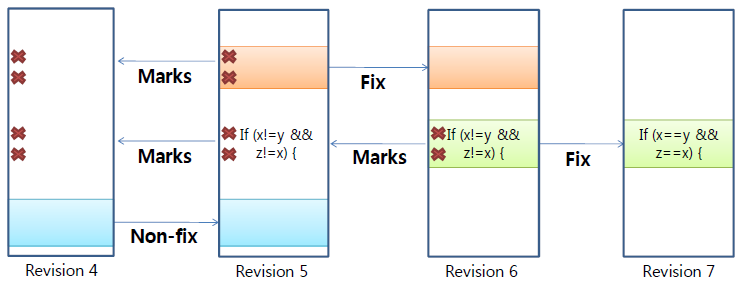
\includegraphics[scale=0.35]{./src/which_warnings_marking.png}
         \caption{Line marking approach}\label{which_warnings:marking}
         \end{subfigure}
     \end{subfigure}%
     \begin{subfigure}{0.4\textwidth}
         \centering
         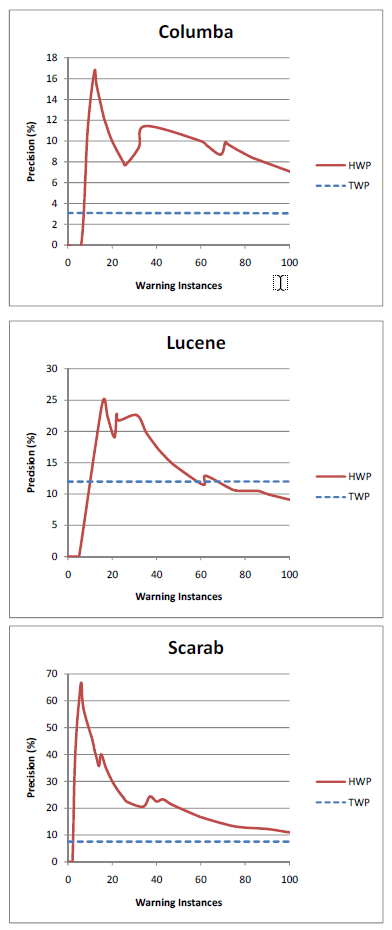
\includegraphics[scale=0.5]{./src/which_warnings_results.png}
         \caption{Line marking approach}\label{which_warnings:results}
     \end{subfigure}
 \end{figure}


 Ruthruff et al. \cite{actionable_sa} use \textit{logistic regression} models to not only reduce the number of false positives in the output of SA tools, but also to predict actionable warnings. Warnings are not always acted on by developers even if they reveal true defects. The reason may be that the defects may have little impact and require significant effort for little perceived benefit. Furthermore, they introduce a statistical methodology for discarding features with low predictive power and thus avoiding the capture of expensive data. Information to build the models is mainly drawn from: (a) light-weight code complexity metrics for post-release bug prediction, (b) file (history) information to predict fault counts within individual files. The features include the history of warnings, source code characteristics, churn factors, and warnings descriptors (\cref{act:metrics}).

 Their screening methodology, for selecting an independent subset of predictor features, consists of up to four stages, and attempts to identify at least six predictive features. The stages respectively consider 5\%, 25\%, 50\%, 100\% of the warnings, continuously removing features with low predictive power. One of the reasons to consider this cost-effective approach is that it may be desirable to rebuild the models at different points in time, either because a significant number of new warnings have been reported, or the codebase has undergone substantial change.

 By considering a sample of around 1600 warnings (inspected by two engineers), and by using different models (with resulting different features) for classifying true positives and actionable warnings, they achieved an accuracy of 85\% for the former, and 70\% for the later (\cref{act:results}).

 \begin{figure}[H]
     \begin{subfigure}{.5\textwidth}
         \centering
         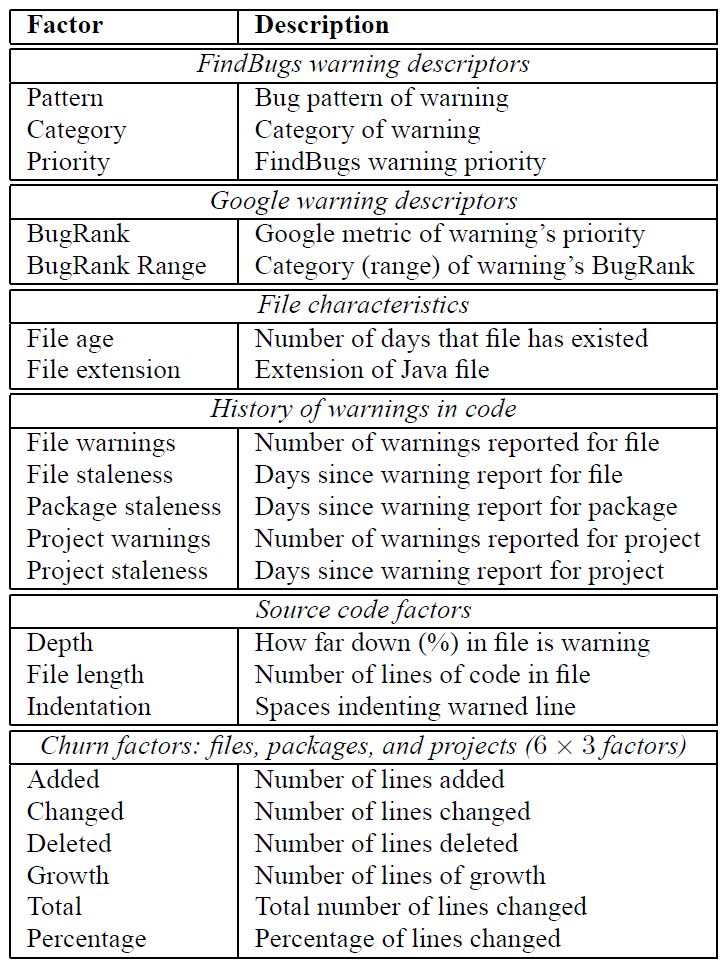
\includegraphics[scale=0.3]{./src/actionable_warnings_metrics.png}
         \caption{Some of the features considered for building the models}\label{act:metrics}
     \end{subfigure}%
     \begin{subfigure}{.5\textwidth}
         \centering
         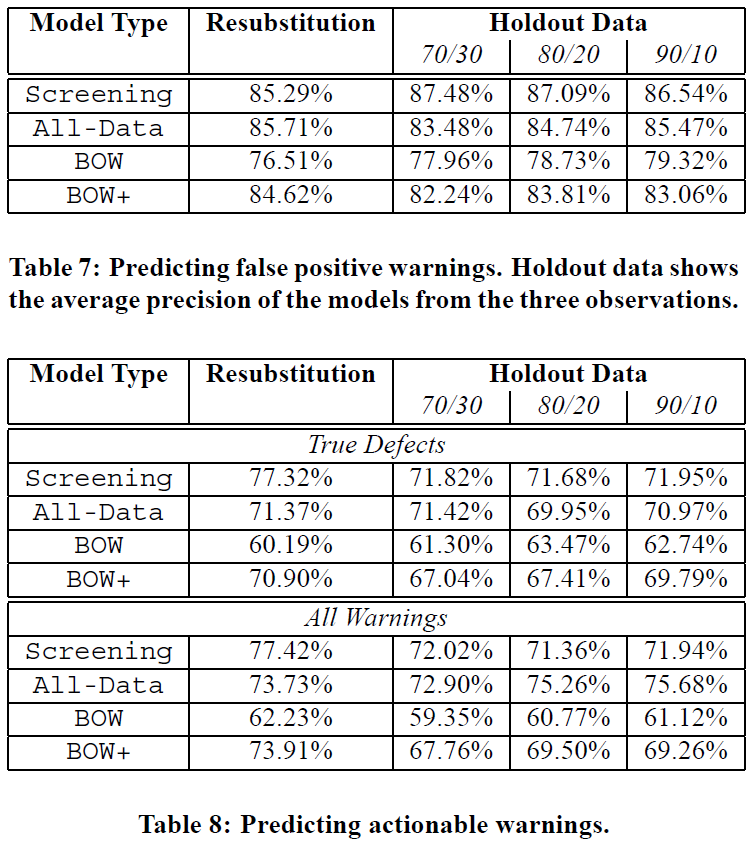
\includegraphics[scale=0.3]{./src/actionable_warnings_results.png}
         \caption{Results for predicting true positives and actionable warnings}\label{act:results}
     \end{subfigure}
 \end{figure}


 Hanam et al. \cite{alert_patterns} present a method for differentiating actionable and unactionable alerts by finding alerts with similar code patterns (alerts with similar patterns are probably of the same type). They use a feature vector based on code characteristics at the site of each SA alert along with a classifier to build a model for predicting AA. They introduce the notion of \textit{alert patterns}, source code patterns employed by developers that are unactionable but are repeatedly flagged by SA tools (or similarly always actionable).

 To extract features from the site of the warning (and near it), lightweight program slicing is used. Backwards slicing is used to detect which statements could have affected the outcome of the seed statement (place of the alert). To speed up the slicing process, all external classes are excluded from the analysis and the depth is limited to the 5 nearest statements prior to the seed.

 By using the source code history of three projects to train and test their approach, they achieve considerably better results than the default ranking of a SA tool (57 vs 19 AA in the top 20\% of the alert list), and a slight improvement (6\%) than the existing techniques.

 \begin{figure}[H]
     \begin{subfigure}{.5\textwidth}
         \centering
         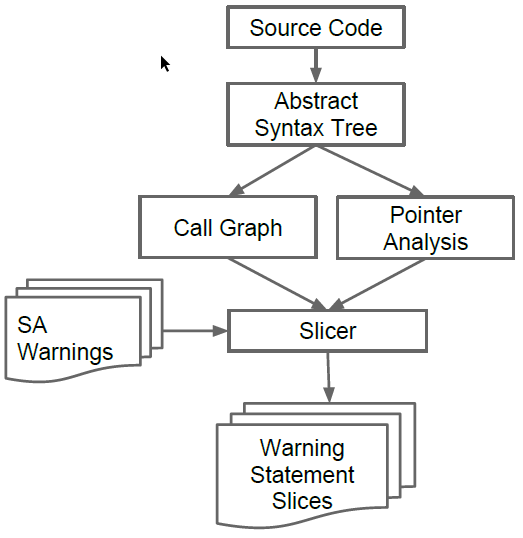
\includegraphics[scale=0.3]{./src/alert_patterns_slicing.png}
         \caption{Method for generating slices}\label{alert_patterns:slicing}
     \end{subfigure}%
     \begin{subfigure}{.5\textwidth}
         \centering
         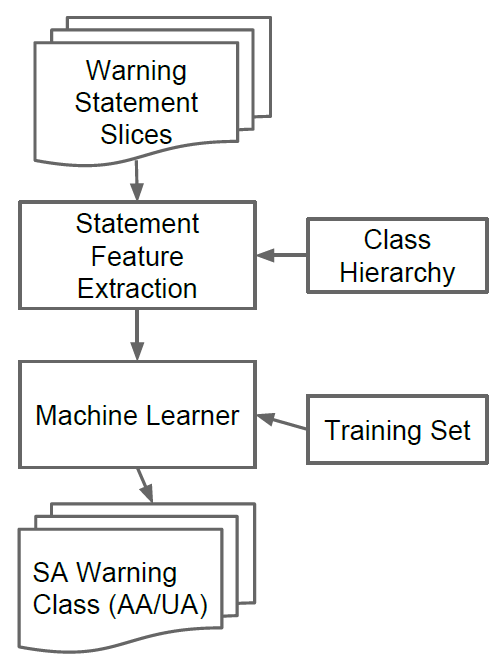
\includegraphics[scale=0.3]{./src/alert_patterns_workflow.png}
         \caption{Workflow for classifying alerts}\label{alert_patterns:workflow}
     \end{subfigure}
 \end{figure}


 Venkatasubramanyam and Gupta \cite{incremental_sa} propose an incremental and lightweight approach to detect coding violations by using a learning system. They track warnings through the version history to detect patterns and determine which SA rules are important (and must be enabled). Their approach focuses on differential code analysis (filter/identify violations happening only on new parts of code), and on learning from the experts.

 Their methodology (\cref{incremental_sa:workflow}) consists of database that continuously stores information about SA rules. The initial version is build by mining (at least) the last three version of the software under analysis. To train the classifier (learning system) different features are used: patterns of code where SA violations are reported, impact of the violations on code quality, confidence level of the rules (probability that a rule gives a false positive), most commonly committed errors (reflecting the developers pattern of coding) and the most recently committed errors.

 New code changes made by developers are checked against the database. By using a patterns matching algorithm that compares new code with the patterns saved in the database, possible bugs can be detected. This approach potentially permits to run the SA tools less frequently, since code violations can be suggested by comparing against past saved patterns. They also suggest using \textit{first order logic} for capturing the context around rule violations and thus learning what factors produce a false/true positive.

 \begin{figure}[H]
     \centering
     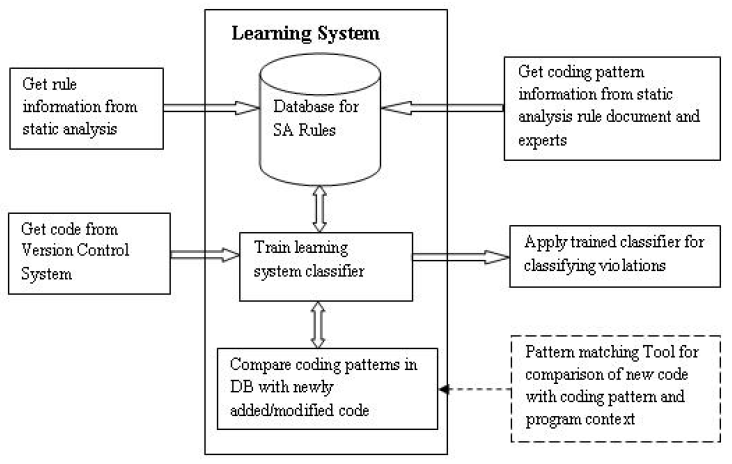
\includegraphics[scale=0.3]{./src/incremental_sa_workflow.png}
     \caption{Workflow for incremental violation detection}\label{incremental_sa:workflow}
 \end{figure}


 Heckman and Williams \cite{model_building_actionable} present a generic approach for building actionable alert machine learning models and provide a comparative study of different algorithms tested of two Java systems. Their initial feature set consists of 51 alert characteristics originating from alert type and history, software metric, software history and source code churn.

 To collect data, they check out and build the program for each chosen revision (in practice they did that once in every 25 revisions) and collect alerts and their characteristics. Starting from the first revision, the sets of alerts between two revisions are compared, collecting information when alerts are opened and closed (and thus classifying them as actionable or unactionable).

 By trying different feature reduction strategies and different machine learning algorithms, they provide results for two systems. The number of selected alert characteristics ranged from 3/4 to 13/14 and both projects had 5 distinctive sets. That shows that the set of AC needs to be tailored for each project. The average metrics for all models (\cref{model_building:results}) show very good results. The difference between selected ACs and
 the best models between projects suggests that false positive mitigation models should be project-specific.

 \begin{figure}[H]
     \centering
     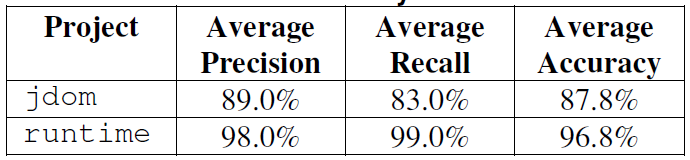
\includegraphics[scale=0.3]{./src/model_building_results.png}
     \caption{Average metrics for all models}\label{model_building:results}
 \end{figure}


 Liang et al. \cite{automatic_training_set} propose an automatic approach (\cref{automatic_training_set:workflow}) for constructing an effective training set for warning prioritization algorithms. They introduce the notion of "generic-bug-fix revisions" vs. "project-specific-bug revisions", which differentiate bug-fixing lines depending on the sort of bug that they deal with. SA tools are designed to catch generic bugs that are applicable to all projects, while most of the bugs are domain (project) specific. By restricting the training set to only those set of bugs that can be caught by the tools, models can be trained better and a higher accuracy can be reached.

 To identify generic-bug-fix revisions, they first limit the revision size to an empirically derived value (max 4 files changed). Then, they analyze the revision messages and using a natural language processing approach compare them against generic bug descriptions (by SA tools). If the similarity of these messages is above a certain threshold and the number of changed files is under the predefined limit, the revision is marked as a generic-bug-fix. To identify the generic-bug-related lines of a specific revision X, they start by analyzing all older revision than X, and backwardly calculate lines that were already present at X, when they were later changed by a generic-bug-fix revision.

 Using a \textit{K-Nearest Neighbor} classifier (trained on the first half of the revisions) paired with a feature selection algorithm, they achieve significantly better result than the tool output, especially in the first 20 warnings range. They found that using multiple SA tools gives a better result than single tool models (\cref{automatic_training_set:multiple_single}). The type training set has also an effect in the final results, models trained only with the project under analysis performed worse that models trained with extra projects (\cref{automatic_training_set:inter_intra}). That adding inter project data (at least in the case of open source projects) has a positive effect in the model predictions can be explained with the choice of focusing only on generic-bug-fix revisions.

 \begin{figure}[H]
     \begin{subfigure}{0.5\textwidth}
         \centering
         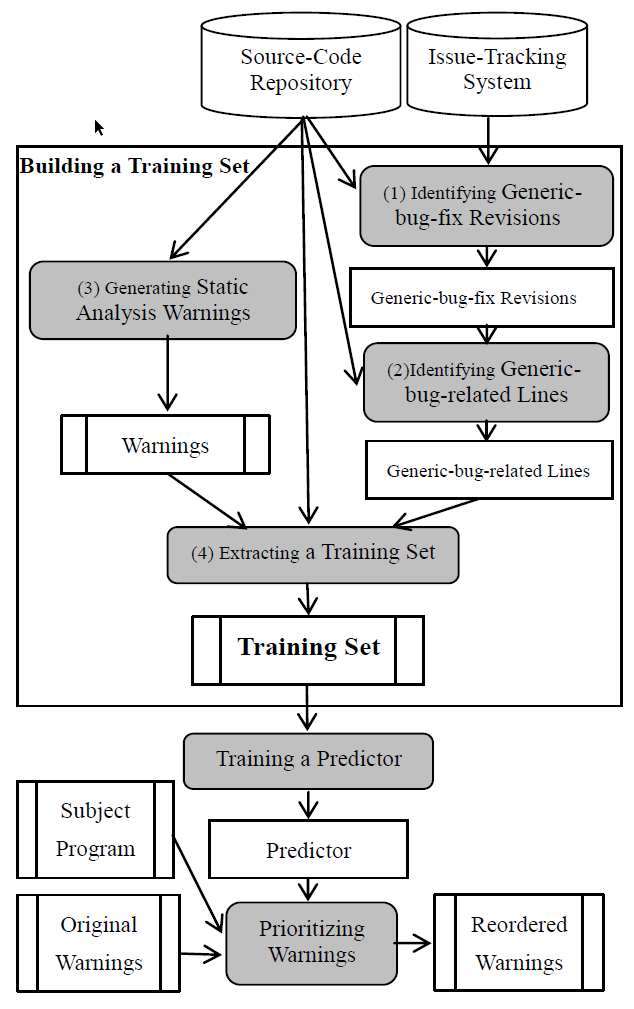
\includegraphics[scale=0.3]{./src/automatic_training_set_workflow.png}
         \caption{Workflow for constructing a training\\ set and a model}\label{automatic_training_set:workflow}
     \end{subfigure}%
     \begin{subfigure}{0.5\textwidth}
         \begin{subfigure}{.5\textwidth}
             \centering
             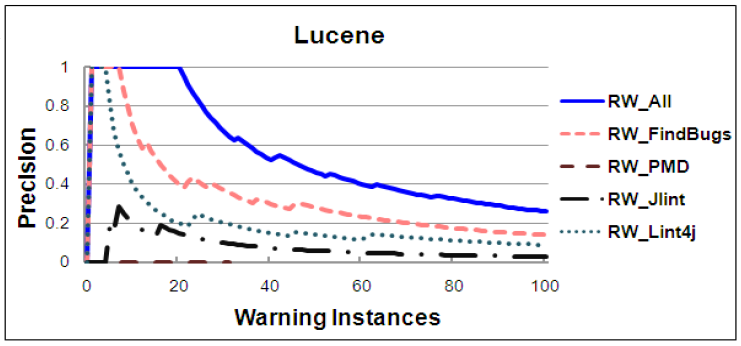
\includegraphics[scale=0.35]{./src/automatic_training_set_results1.png}
             \caption{Multiple vs. single tool results using training set}
             \label{automatic_training_set:multiple_single}
         \end{subfigure}\\
         \begin{subfigure}{.5\textwidth}
         \centering
         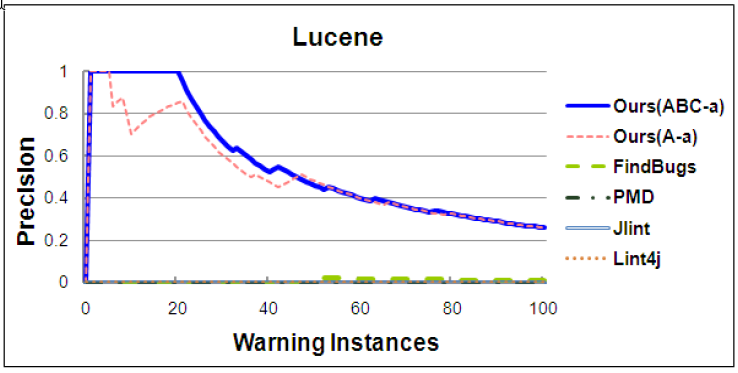
\includegraphics[scale=0.35]{./src/automatic_training_set_results2.png}
         \caption{Intra (A-a) vs inter (ABC-a) project training}
         \label{automatic_training_set:inter_intra}
         \end{subfigure}
     \end{subfigure}
 \end{figure}


 \subsubsection{Multiple Tools}

 Flynn et al. \cite{multiple_classification} use \textit{Alert Fusion} (unifying alert information from different tools) and different classifiers to classify alerts as expected true positive (e-TP), expected true negative (e-TN) and indeterminate (I). The e-TP alerts are separately prioritized for code repair and the I-alerts are automatically ranked based on classifier confidence and a cost metric to fix the code flaw. 

 The authors used a total of 354 manually audited SA alerts, which there then mapped to standardized coding rule violations (CERT). Different types of classifiers were used, using different portions of data: trained to detect a single rule violation, trained for a single programming language, and all rule classifiers. The results vary from around 80 to 90\% accuracy, depending on the classifier type. The reliability of some of the results is doubtful since one of the major problems of the study was a lack of data.

 \begin{figure}[H]
     \begin{subfigure}{.5\textwidth}
         \centering
         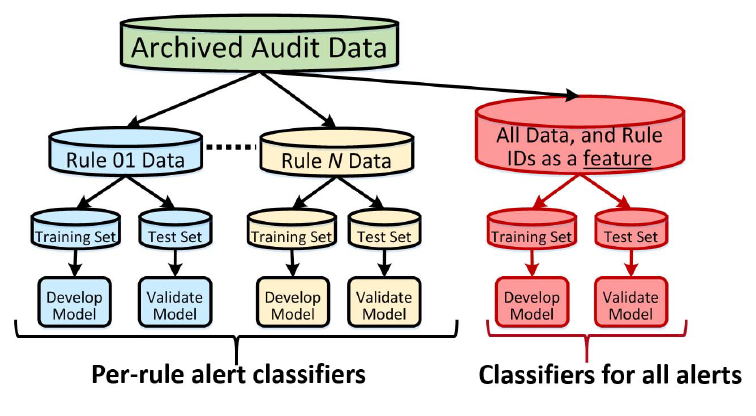
\includegraphics[scale=0.3]{./src/multiple_classifiers_workflow.png}
         \caption{Workflow of building classifiers}\label{multiple_classifiers:workflow}
     \end{subfigure}%
     \begin{subfigure}{.5\textwidth}
         \centering
         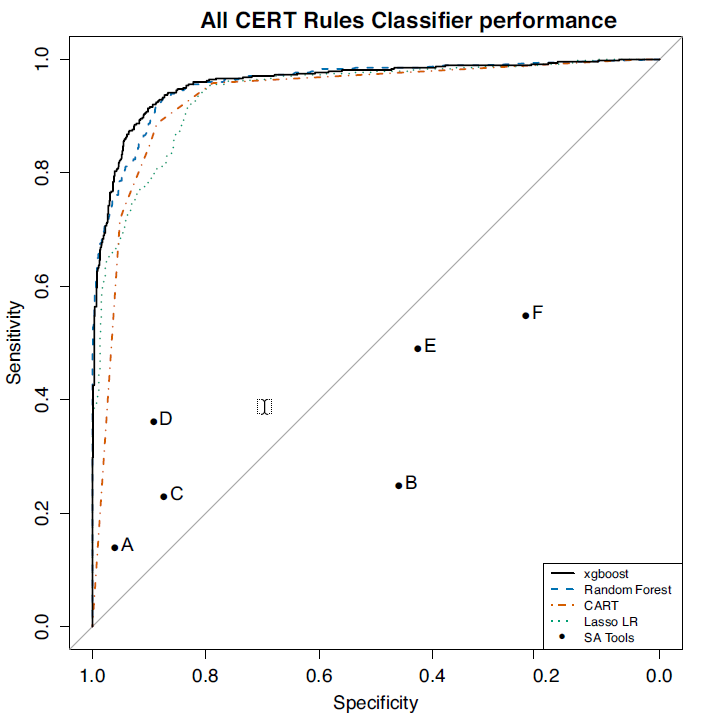
\includegraphics[scale=0.3]{./src/multiple_classifiers_resulst.png}
         \caption{Results of all-rules classifiers}\label{multiple_classifiers:results}
     \end{subfigure}
 \end{figure}


 Ribeiro et al. \cite{multiple_ensemble} aim to reduce the false positive rate of an ensemble of static analyzers by using \textit{Decision Trees} and \textit{AdaBoost}. The goal is to make possible to combine the strengths of different analyzers without suffering too much from false positives. Their approach ignores source code characteristics, making it possible to be applied without any pre-processing step on the codebase.

 They use \textit{Juliet}, a synthetic C/C++ test suite which contains specific flaws with links to program code, to train and test the classifiers (see \cref{multiple_classifiers_ensemble:warnings} for the results of different tools on the set of selected test cases). The features to train the model include the tool name, number of warnings per file, warning category, number of neighboring warnings, number of warnings per file, and a boolean feature for each of the static analyzers.

 By combining weak decision tree classifiers with AdaBoost, they can reach a mean acccuracy of 80\% with a hundred trees, with precision and recall around 68\% and 96\% respectively. The ranking is done by sorting the warnings according to the probability assigned by the model, achieving a five time improvement over random ordering. The most important features in the classifier were the number of warnings per file and the tool name.

 \begin{figure}[H]
     \begin{subfigure}{.5\textwidth}
         \centering
         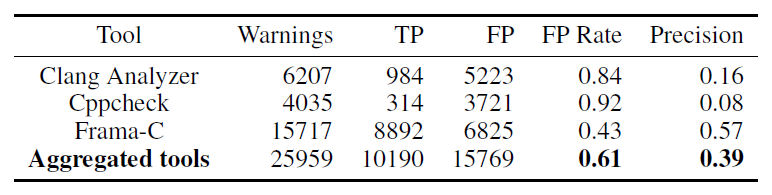
\includegraphics[scale=0.3]{./src/multiple_classifiers_ensemble_warnings.png}
         \caption{Labeled warnings per tool (from the extracted list of Juliet)}\label{multiple_classifiers_ensemble:warnings}
     \end{subfigure}%
     \begin{subfigure}{.5\textwidth}
         \centering
         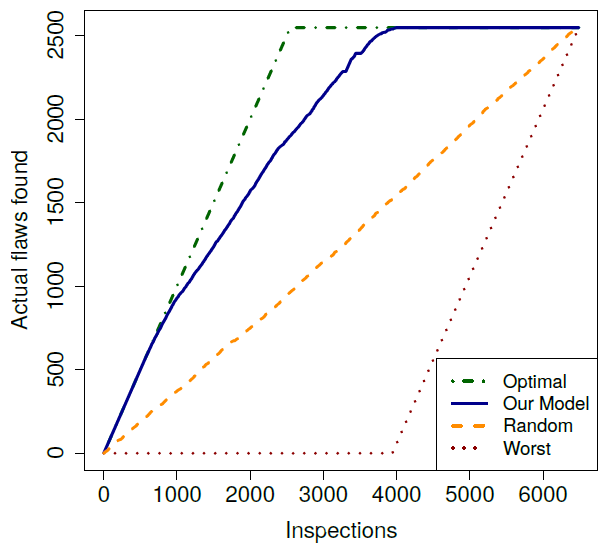
\includegraphics[scale=0.3]{./src/multiple_classifiers_ensemble_results.png}
         \caption{Results of the classifier}\label{multiple_classifiers_ensemble:results}
     \end{subfigure}
 \end{figure}


 \subsubsection{Literature review papers}

 Heckman and Williams \cite{literature_actionable} perform a systematic review of \textit{Actionable Alert Identification Techniques} (AAIT). The goal is to make an informed decision which AAIT to pair to an SA tool, in order to present relevant warnings to the tool users. An actionable alert is defined as an important, fixable anomaly. Different studies have estimated the amount of unactionable alerts ranging from 35\% to 91\%. The authors divide the tools into different categories, based on input type, approach used, and evaluation method.

 The categories of artifacts used by AAIT's are divided into five main categories: (a) alert characteristics (type, location), (b) code characteristics (metrics), (c) source code repository metrics (code churn), (d) bud database metrics, (e) dynamic analysis metrics (extracted during code execution). Most AAIT's combine more than one of these input categories.

 Approaches followed by AAIT's fall into seven main categories: (a) alert type selection (selecting altert types that are the most relevant for a codebase), (b) contextual information (limiting SA tools only to parts of code where that they can analyze well), (c) data fusion (combining multiple SA tools), (d) graph theory (system dependency graphs or repository history of changes), (e) machine learning, (f) mathematical and statistical models, (g) test case failures (generate test cases that demonstrate faults in the warning location). 

 Evaluation methodologies are divided into six categories: (a) baseline comparison (use a standard baseline), (b) benchmarks, (c) comparison to other AAIT's, (d) random and optimal order comparison, (e) train and test, (f) other.
 Classification AAIT's are evaluated using typical metrics as precision, recall, accuracy, and false positive rate, while Prioritization AAIT's are evaluated using correlation coefficients, statistical tests (chi-square), improvements over random, AUC etc..\\\\


 Muske and Serebrenik \cite{survey_approaches} perform a systematic review of SA alarm handling techniques (\cref{survey:papers}). They define \textit{handling of alarms}  as: (a) post-processing to reducing the manual inspection effort (using correlation, clustering, ranking...), and (b) supporting manual inspection of alarms.

 Seven categories for identifying alarms are defined (\cref{survey:categories}): (a) clustering, (b) ranking, (c) pruning, (d) false positive elimination, (e) combination with dynamic analysis, (f) simplifying inspections, (g) design of light-weight SA tools (\textit{LSATs}).

 In \textit{clustering}, alarms are partitioned into several groups based on similarity/correlation. There are two sub-categories: sound clustering, where there is a guarantee of certain dependencies among clustered alarms, and unsound clustering, where there are no guarantees on dependencies/relationships. 
 In \textit{ranking}, alarms are prioritized and those more likely to be errors are output at the top of the list. Different techniques can be used to support ranking, such as statistical models, history of alarm fixes, user feedback etc... 
 In \textit{pruning}, alarms are classified as actionable or non-actionable. Machine learning techniques can be used to classify the alarms (using patterns from surrounding code and syntactic/semantic differences), or alarm delta identification can be used identify the alarms that are newly generated (useful for legacy code). 
 In \textit{false positive elimination}, more precise techniques like model checking and symbolic execution are used to eliminate false positives. This approach is more precise and automatic but faces the issues of non scalability and poor performance.
 In \textit{combining dynamic and static analysis}, SA alarms are checked if they are true errors. SA has been combined with test-case generation or slicing to find errors or extract more precise information.
 In \textit{simplifying manual inspection}, approaches are used to help the user in alarm inspection by making inspections more automatic/systematic. Different techniques are used, from rule and checklist based approaches, to improved visualisation, to automatically deriving possible alarm causes.
 In \textit{designing LSATs}, light-weight, scalable and shallow analysis tools are built to avoid generation of a large number of alarms. However there are no guarantees that all defects of a type will be uncovered.

 \begin{figure}[H]
     \begin{subfigure}{1\textwidth}
         \centering
         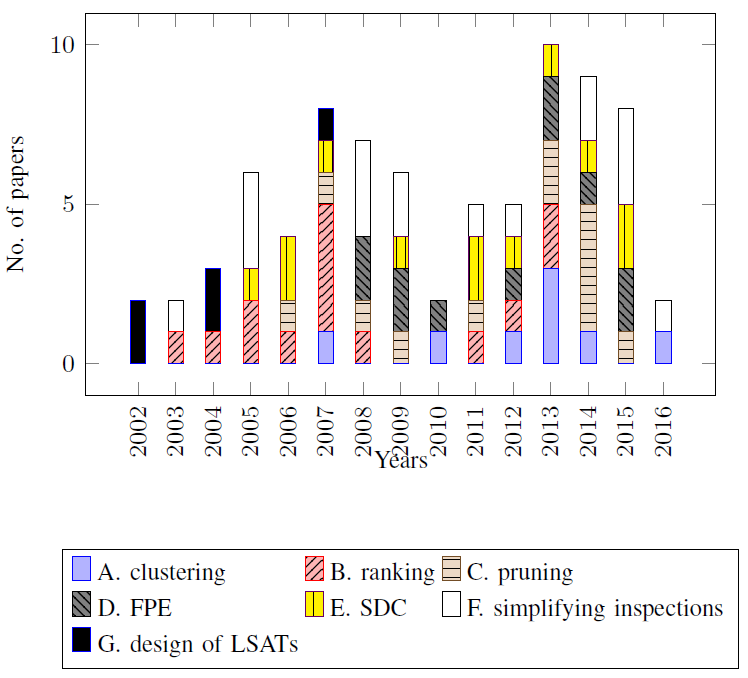
\includegraphics[scale=0.4]{./src/survey_sa_papers.png}
         \caption{Number of relevant papers per year and category}\label{survey:papers}
     \end{subfigure}\\
     \begin{subfigure}{1\textwidth}
         \centering
         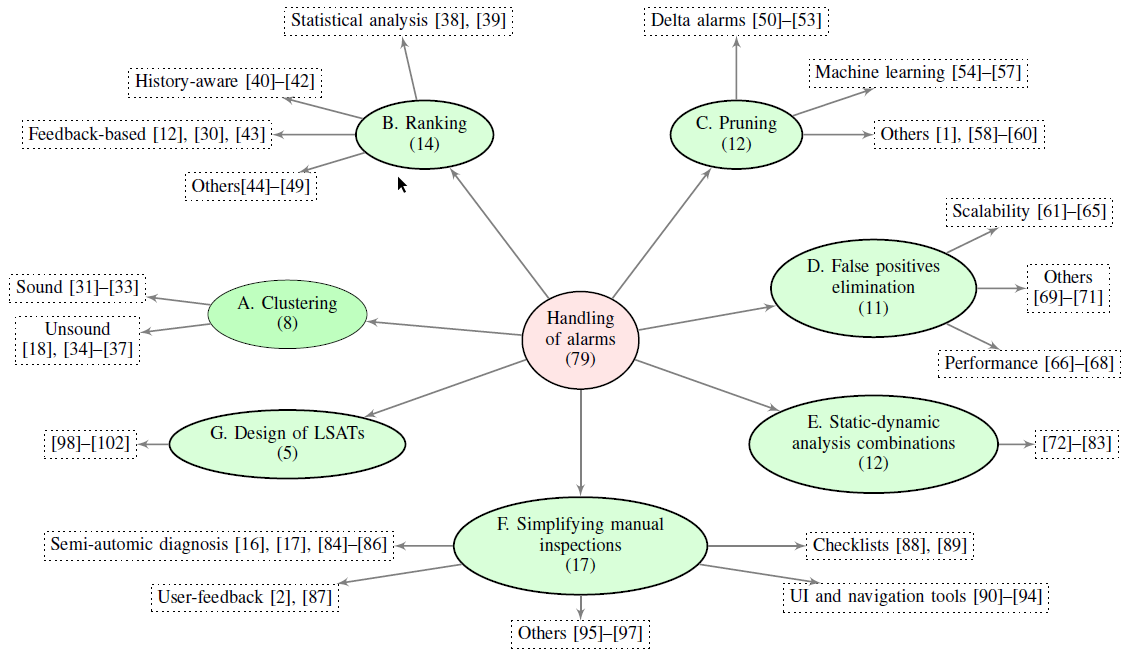
\includegraphics[scale=0.4]{./src/survey_sa_categories.png}
         \caption{Summary of the approaches}\label{survey:categories}
     \end{subfigure}
 \end{figure}


\subsubsection{Comparative studies}

Heckman and Williams \cite{comparative_heckman} perform a comparative study of six alert ranking techniques on the \textit{Faultbench} dataset: (a) Actionable Prioritization models that are based on the assumption that alerts sharing a type/location are like to be all actionable or non-actionable, (b) Alert Type Lifetime models that prioritize alert types by their average lifetime (important alerts are fixed quickly), (c) Check 'n Crash that automatically generates unit test cases and checks if the test fails (alert is then considered actionable), (d) History-Based Warning Prioritization models that uses commit messages and code changes in the source code repository to prioritize alert types, (e) Logistic Regression models that are trained on thirty-three alert characteristics and predict the probability of an alert being actionable, (f) Systematic Actionable Alert Identification that collects a number of alert characteristics and tries to find the best subset of these characteristics and the best machine learning models that optimizes accuracy and precision.

On each of the three test projects of the benchmark, there is a different winner (based on accuracy), with Systematic Actionable Alert Identification and Logistic Regression models that generally perform better. There is also a trend where precision and recall decrease with the amount of analyzed revisions (70, 80 or 90\%). That can be explained by the fact that the balance between actionable and unactionable alerts is heavily shifted to the later. This trend can also be explained by the fact that these techniques can be better at identifying unactionable alerts than actionable alerts.


Allier et al. \cite{compare_framework} perform a comparison of different ranking algorithms based on their effort metric: average number of alerts to inspect to find an actionable one. They also focus on two other research questions, whether its better to rank alerts individually or alert types, and if there is a performance difference between statistical ranking methods and ad-hoc ones. They test six raking approaches ( six Java and Smalltalk systems): Aware, FeedbackRank and Z-Ranking which mainly use alert type and location, RPM that uses logistic regression with thirty-three alert characteristics, AlertLifeTime that prioritizes alerts on type and lifetime, and EFindBugs which prioritizes alert types based on their defect likelihood.

They found out that Aware and FeedbackRank perform significantly better than the other ranking approaches. In addition individual alert raking algorithms performed better than those that rank alert types. Also they did not find a clear distinction in performance between statistical and ad-hoc approaches.


 \subsection{Bug Prediction}

 Nagappan et al. \cite{mining_metrics} use code complexity metrics to predict the likelihood of \textit{post-release} defects for new entities (failures that occurred in the field six months after the release). Although, according to their findings, these metrics are correlated to failure prone entities, there is no universal set of metrics that produces the best results. As a consequence, principal component analysis is used to choose the optimal set of features for a particular project. Information from bug databases and historical data is used to select the appropriate metrics.

 By analyzing a set of five large scale projects, they discovered the following results: (a) for each project a set of metrics can be found that correlates with post-release defects, (b) there is no single et of metrics that fits all projects, (c) predictors build using \textit{PCA} are useful for building regression models that predict post-release defects, (d) predictors are only accurate when obtain from the same or similar projects.

 This approach can be generalized to predict arbitrary measures of quality, as long as we can extract the right information from the project's history. The general workflow is the following: decompose system in entities, build a function that assigns a quality measure to an entity, have a set of metrics and a metric functions that assigns a value to each entity, determine correlation of metrics to the quality measure and use PCA to select the most relevant set, use the principal components to predict quality of new entities.

 % \begin{figure}[H]
 %     \centering
 %     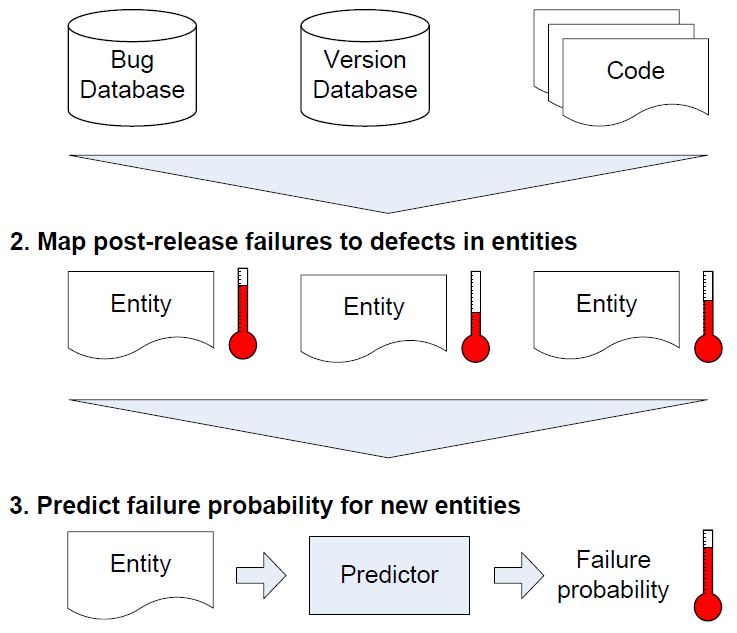
\includegraphics[scale=0.3]{./src/mining_metrics_overview.png}
 %     \caption{Some of the features considered for building the models}\label{mining:overview}
 % \end{figure}

 \begin{figure}[H]
     \begin{subfigure}{.5\textwidth}
         \centering
         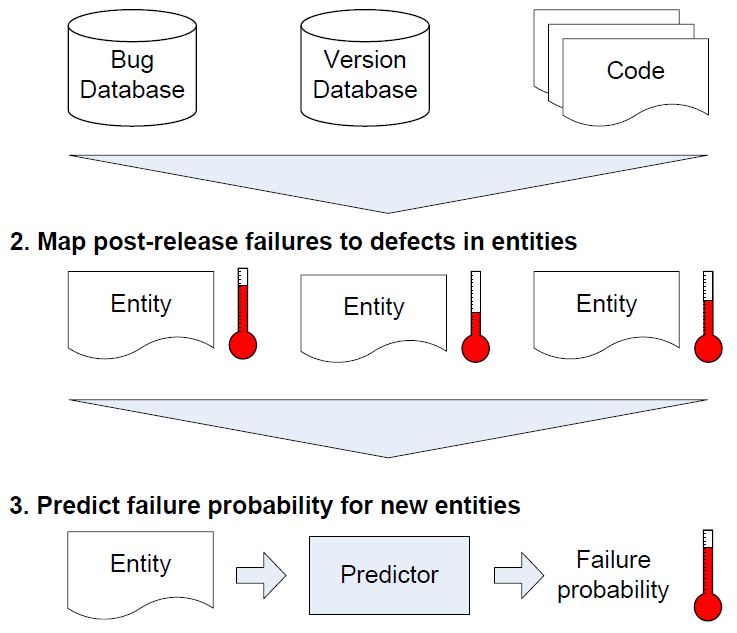
\includegraphics[scale=0.3]{./src/mining_metrics_overview.png}
         \caption{Workflow for predicting defects on new entities}\label{mining:overview}
     \end{subfigure}%
     \begin{subfigure}{.5\textwidth}
         \centering
         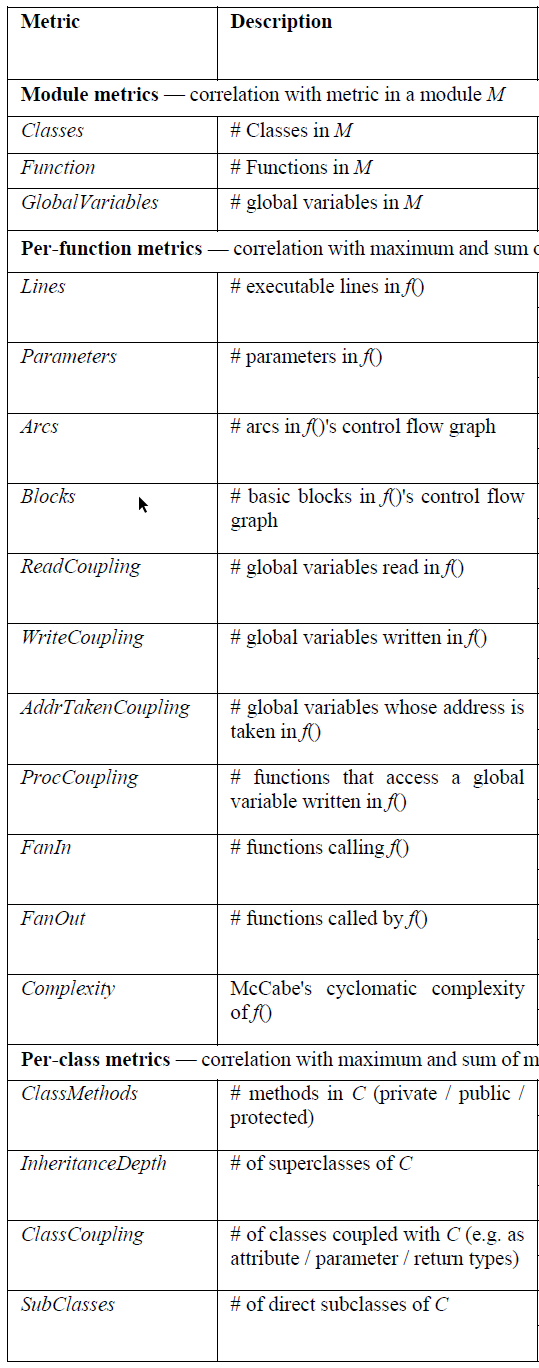
\includegraphics[scale=0.2]{./src/mining_metrics_metrics.png}
         \caption{The set of complexity metrics considered}\label{mining:metrics}
     \end{subfigure}
 \end{figure}


 Giger et al. \cite{prediction_method} present bug prediction models at method level. In comparison to previous file or module level techniques, this increases the granularity of the prediction and thus reduces manual inspection (developers don't have to inspect a whole file). 

 The models are based on source code metrics that are applicable on method level (\cref{method_prediction:metrics}) while change metrics are based on fine-grained operations extracted from AST comparisons (tree edit operations needed to transform one AST into the other, combined with semantic information from the source code, \cref{method_prediction:ast}).

 By using an extensive test set of multiple open source Java projects and by labeling each method as bug-prone or not bug-prone (using historical VCS data) they were able to measure the efficacy of different classifiers. The classifiers were trained with both source and change metrics and each separately. The source metrics alone performed significantly worse than the other two and suffer from low precision values (around \%50). The change metrics (combined or not with the source ones) perform significantly better (> 80 \% precision) and the type of classifier does not significantly affect the results (\cref{method_prediction:results}).

 \begin{figure}[H]
     \begin{subfigure}{.5\textwidth}
         \centering
         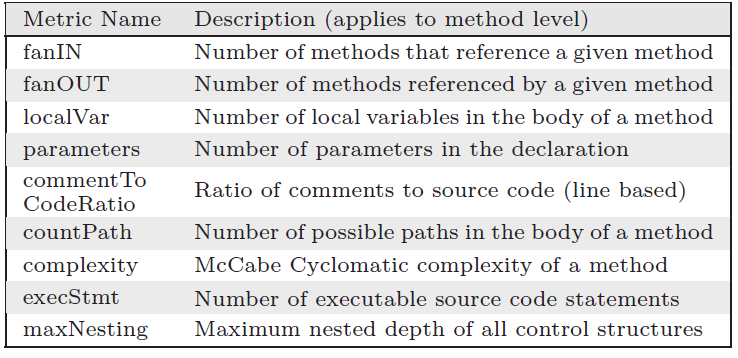
\includegraphics[scale=0.3]{./src/method_prediction_metrics.png}
         \caption{Method level metrics used for prediction}\label{method_prediction:metrics}
     \end{subfigure}%
     \begin{subfigure}{.5\textwidth}
         \centering
         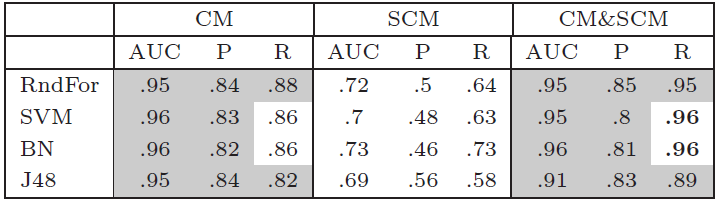
\includegraphics[scale=0.4]{./src/method_prediction_results.png}
         \caption{Precision, recall and AUC results for the metric sets}\label{method_prediction:results}
     \end{subfigure}\\
     \begin{subfigure}{\textwidth}
         \centering
         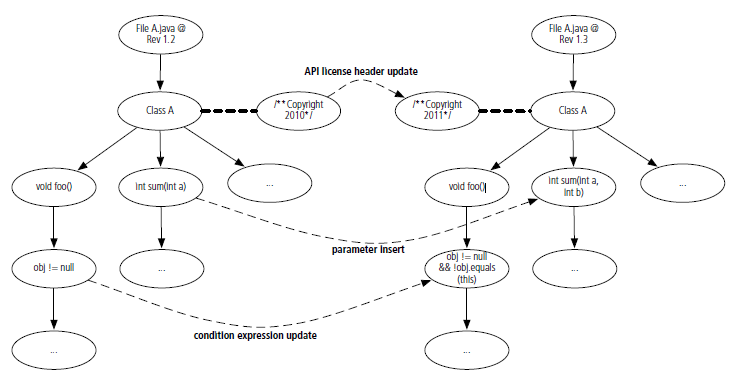
\includegraphics[scale=0.4]{./src/method_prediction_ast.png}
         \caption{Fine grained code changes extracted from AST comparisons}\label{method_prediction:ast}
     \end{subfigure}  
 \end{figure}


 Wang et al. \cite{predict_deeplearning} leverage deep learning to automatically learn semantic features from source code. The aim is to apply this knowledge into defect prediction, which traditionally uses syntactic features to build the models. In order to make accurate prediction, the features need to be discriminative, but traditional features cannot distinguish code regions with different semantics (see for example \cref{deeplearning:example}).

 A Deep Belief Neural Network is used to learn the semantic features from input vectors that contain tokens extracted from the AST's (code is parsed into tokens, tokens are then mapped into integers, which then form the vectors). Three main categories of AST nodes are extracted: a) nodes of method invocations and class instance creations, b) declaration nodes, c) and control flow nodes (see \cref{deeplearning:workflow} for the general workflow).

 To handle noise in data, the edit distance between the token sequences along with the \textit{Closest List Noise Identification} approach is used (compare instance label against its k-nearest neighbors). Additionally, infrequent tokens are filtered out of the training process.

 The DBN is tested against models trained with traditional features and models trained with the AST nodes. As can be seen from \cref{deeplearning:results}, the DL approach outperforms the traditional methods, with an average improvement in precision and recall of 14\% and 11\% respectively.

 \begin{figure}[H]
     \begin{subfigure}{1\textwidth}
         \centering
         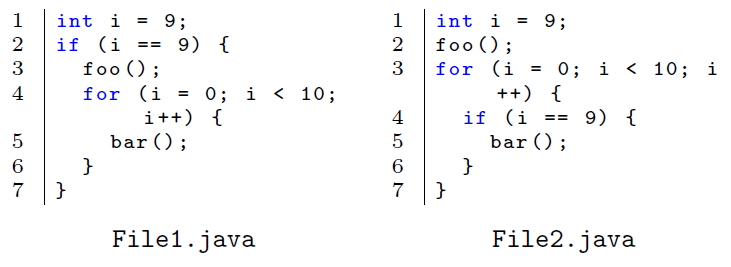
\includegraphics[scale=0.5]{./src/deeplearning_example.png}
         \caption{Example of programs with same syntax (tokens) but different semantics}\label{deeplearning:example}
     \end{subfigure}\\
     \begin{subfigure}{\textwidth}
         \centering
             \makebox[\textwidth]{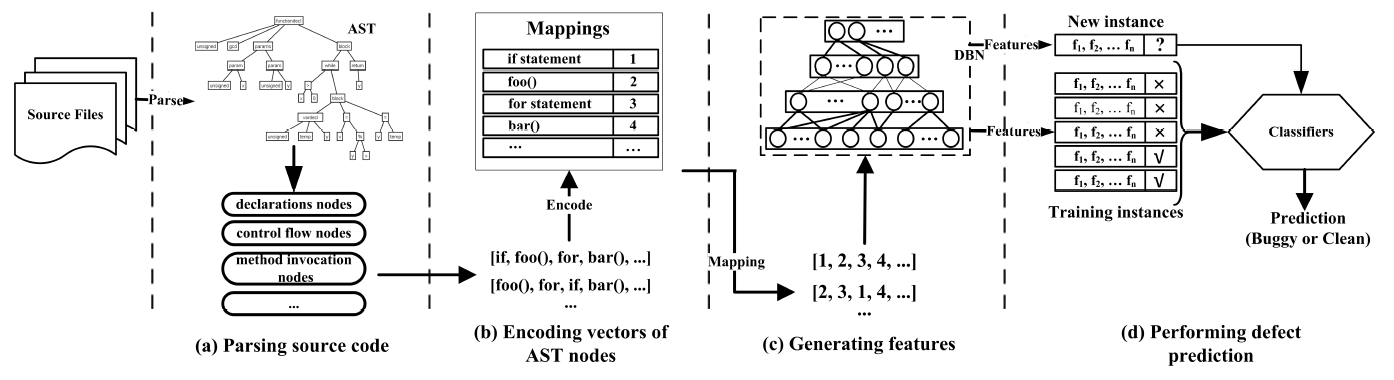
\includegraphics[scale=0.5]{./src/deeplearning_workflow.png}}%
         \caption{Workflow for the semantic learning process}\label{deeplearning:workflow}
     \end{subfigure}\\
     \begin{subfigure}{1\textwidth}
         \centering
         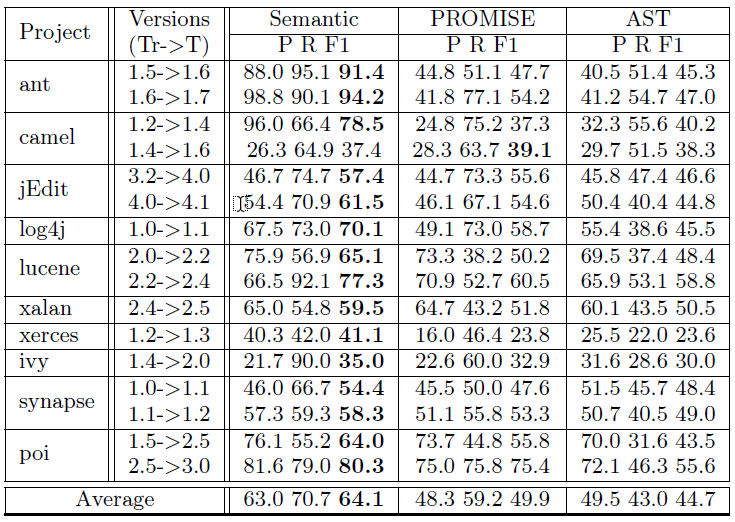
\includegraphics[scale=0.4]{./src/deeplearning_results.png}
         \caption{Precision, recall and F1 score for semantic vs syntactic features}\label{deeplearning:results}
     \end{subfigure}
 \end{figure}


 Yang et al. \cite{dl_jit_prediction} propose a deep learning technique to detect defect-prone changes (just-in-time defect prediction, i.e. inside commits). The advantage of this granularity is that there is a smaller amount of code to check and that it is easy to decide which developer should fix a bug (the one who committed the code). They use a two phase approach: a feature selection phase and a machine learning phase.

 The feature selection phase is to decide the best set of features to use to train the model. The data is pre-processed to in two steps: data is first normalized and then random under-sampling is used to balance the categories of buggy or not buggy changes. Since in logistic regression each feature is calculated independently, new features cannot be created by combining existing ones. For that reason, they leverage \textit{Deep Belief Networks} to generate a more expressive feature set. 

 The logistic regression model is trained with the new feature set and evaluated with a cost effectiveness measure defined as the percentage of bugs that can be discovered by inspecting the top (most relevant) 20\% lines of code. On average 50\% of bugs can be found in the top 20\% LOC, and the feature processing step helps logistic regression achieve better results than previous approaches (\cref{dl_jit:results}).

 \begin{figure}[H]
     \centering
     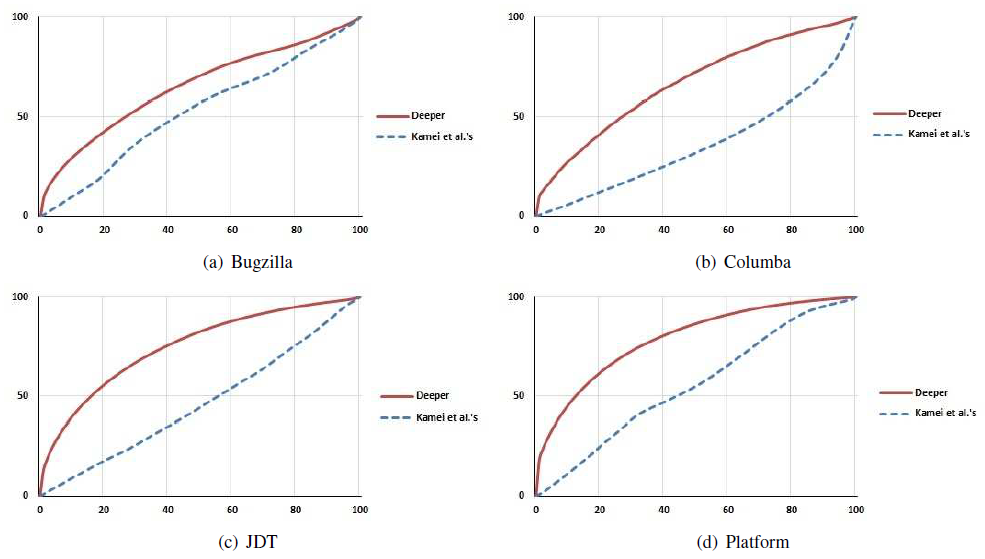
\includegraphics[scale=0.5]{./src/dl_jit_results.png}
     \caption{Improvements over classic logistic regression approach}\label{dl_jit:results}
 \end{figure}



 \subsection{Static Analysis tools in practice}

 Beller et al. \cite{analysis_sa_usage} conduct a large scale evaluation of how SA tools are used in practice in open-source systems. They study the prevalence of SA tools, their configurations and how they evolve.

 By performing a survey on a 36 open-source projects, they found out that most of them used SA tools, with a relevant subset using more that one (\cref{sa_analysis_survey:usage}). Although, most of them run the tools sporadically and without enforcing them.

 A configuration file of a SA tool, shows what rules developers deem important (enable), and what they do not deem important (disabled, perhaps because of a high false positives rate). The contents of a configuration file are hence an important indicator of how developers use SAs and how well the tool’s default settings reflect its use.

 In the analyzed projects, most enabled rules belong to the maintainability category, and only 35\% of the enabled rules belong to a functional category. Both the majority of actively enabled and disabled rules are maintainability-related.

 Most configurations change or reconfigure rules from the default configuration, but typically only one rule. Most changes are small, and a third of them happen in the first week of creation of the configuration. Also, most configuration files never change (\cref{sa_analysis_survey:changes}).

 \begin{figure}[H]
     \begin{subfigure}{1\textwidth}
         \centering
         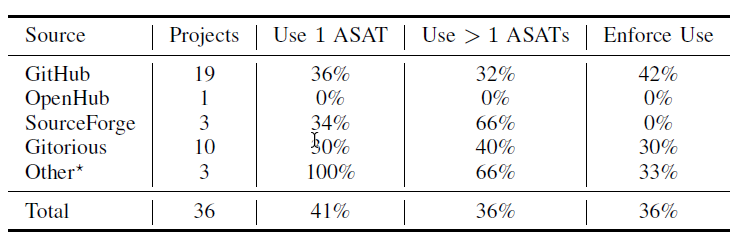
\includegraphics[scale=0.4]{./src/sa_analysis_survey_usage.png}
         \caption{Survey results of 36 open-source systems using SA tools}\label{sa_analysis_survey:usage}
     \end{subfigure}\\
     \begin{subfigure}{1\textwidth}
         \centering
         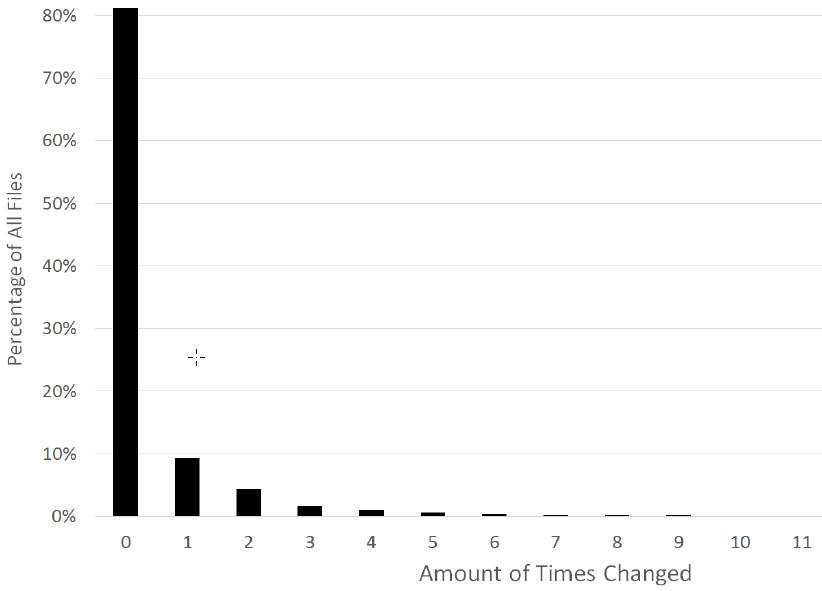
\includegraphics[scale=0.4]{./src/sa_analysis_survey_changes.png}
         \caption{Changes in configuration of SA tools}\label{sa_analysis_survey:changes}
     \end{subfigure}
 \end{figure}


 Imtiaz et al. \cite{how_act_sa} analyze the SA usage of five large open-source systems (the tool is \textit{Coverity}). They study the amount of actionable alerts, time for fixing alerts and the size of fixes.

 They discover that 80\% of alerts belong to 20\% of the alert types and that the actionability rate varies from 27\% to 49\% depending on the project (\cref{how_use_sa:actionable}). Also in the case of actionable alerts, 20\% of the types causes 80\% of the actionable alerts.

 The median lifespan of actionable alerts varies between projects, ranging from 36 to 245 days, and the complexity of code changes is generally low. This means that developers generally take a long time to fix the alerts despite the fixes being low in complexity.

 To increase the developer interaction with SA tools they suggest two solutions: (a) prioritizing the most critical alerts and (b) providing an estimate for the fix effort.

 \begin{figure}[H]
     \begin{subfigure}{1\textwidth}
         \centering
         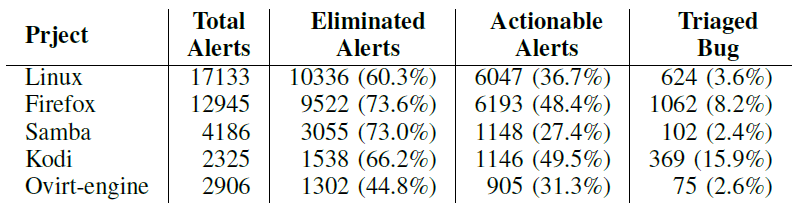
\includegraphics[scale=0.4]{./src/how_use_sa_actionable.png}
         \caption{Actionability results for total alerts}\label{how_use_sa:actionable}
     \end{subfigure}\\
     \begin{subfigure}{1\textwidth}
         \centering
         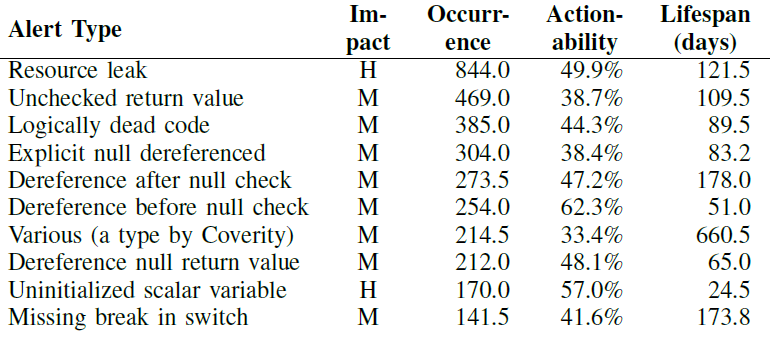
\includegraphics[scale=0.4]{./src/how_use_sa_topalerts.png}
         \caption{Top 10 alert occurrences for C/C++}\label{how_use_sa:top}
     \end{subfigure}
 \end{figure}


 Habib and Pradel \cite{how_many_bugs} study how many of all real-world bugs static bug detectors find. The results of their study show that: (a) static bug detectors find a non-negligible amount of all bugs, (b) different tools are mostly complementary to each other (see \cref{how_many_bugs:partition}), and (c) current bug detectors miss the large majority of the studied bugs.

 The three bug detectors together reveal 27 of the 594 studied bugs (4.5\%). Some of the missed bugs could have been found by variants of the existing detectors, while most of them are domain-specific problems that do not match any existing bug pattern that the SA tool have. By manually analyzing a small subset of 20 bugs, 14 of them were domain-specific and not related to any pattern supported by the checkers, while 6 of them were near-misses that could have been detected with a more powerful variant of the tool.

 They also found that the majority of bug fixes is limited in size and that most bugs are clustered on a small percentage of files (\cref{how_many_bugs:fixsize}).

 \begin{figure}[H]
     \begin{subfigure}{1\textwidth}
         \centering
         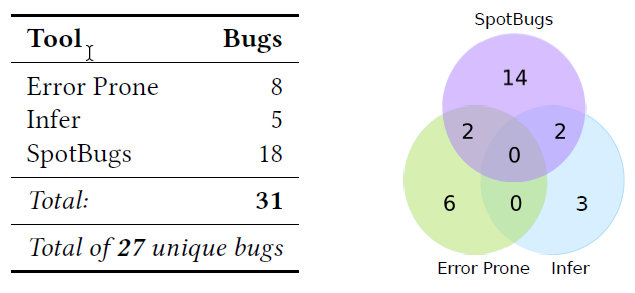
\includegraphics[scale=0.4]{./src/how_many_bugs_partition.png}
         \caption{Distribution of found bugs per tool}\label{how_many_bugs:partition}
     \end{subfigure}\\
     \begin{subfigure}{1\textwidth}
         \centering
         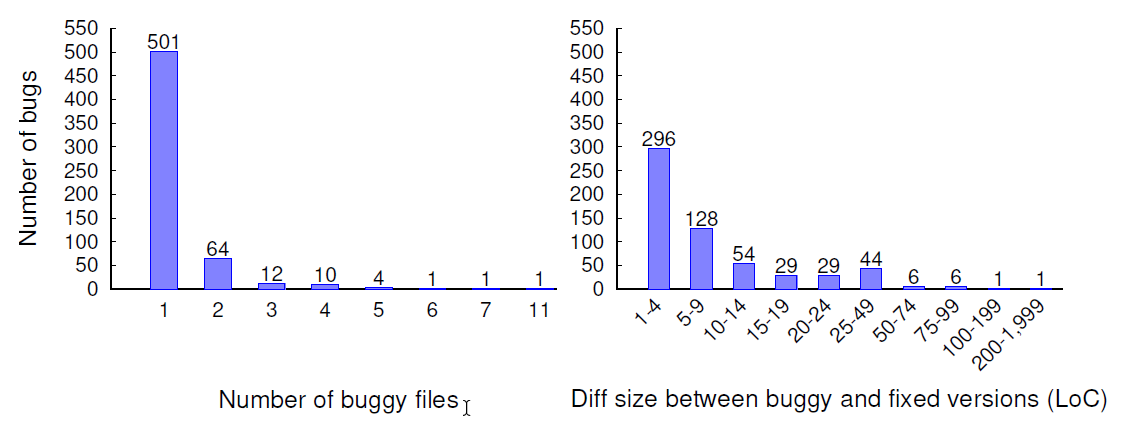
\includegraphics[scale=0.4]{./src/how_many_bugs_fixsize.png}
         \caption{Bugs/file and lines/bugfix}\label{how_many_bugs:fixsize}
     \end{subfigure}
 \end{figure}


 Sadowski et al. \cite{sa_google} provide an overview of the process that Google underwent to increase the developer interaction with SA tools. They list a number of shortcomings that hinder large scale adoption of such tools and suggest solutions that proved effective in their company. 

 The main reasons developers ignore of lose faith in SA tools are: (a) \textbf{no integration in workflow} (most important reason), (b) non actionable warnings, (c) reported bugs do not manifest in practice, (d) suggested bug is too risky/expensive to fix, (e) warnings are not understood.

 Google switched from the dashboard based \textit{FindBugs} tool (whose warnings were mostly ignored for two main reasons: developers lost faith because of false positives or alerts that were not important, and because the warnings came to late in the development workflow), to another better integrated approach.
 According to their findings, reporting issues sooner is better: moving as many checks into the compiler is the way to go. When possible, fixes are suggested or carried out automatically. A second place to show alerts that relate to high impact bugs, is the code review platform (for alerts with no simple fix). Code review is also a good context for reporting relatively less-important issues like stylistic problems or opportunities to simplify code.

 Another key point in making SA tools more valuable for the developers, is integrating their feedback, whether they accept or not the alerts proposed by the tool (for ex. adding a button for each alert \textit{Useful/Not Useful}).
 An additional workflow integration point is \textit{gating commits}: blocking a commit when a check fails (used for check with a low false positive rate).


% \subsection{Available tools}
% Open source tools found:
% \begin{itemize}
%     \item Infer
%     \item CppCheck
% \end{itemize}

% \subsection{Ideas?}
% \begin{itemize}
%     \item \textbf{Feasibility study}: combining different techniques (\cite{survey_approaches}). Pipelining or parallel?
%     \item mine bug messages / fixes to extract useful information?
%     \item use \cite{mining_metrics} to predict actionable warnings
%     \item lightweight local (file level?) execution likelihood
%     \item z-ranking or weighted warnings for cpp core guidelines
%     \item use ignore commands found in code for pruning future warning reports
%     \item see \cite{predict_deeplearning} introduction for a list of feature selection (also links to interesting papers)
%     \item To prune noisy data: mislabeling data detection approach Closest List Noise Identification (CLNI).
%     \item deep learning to classify warnings
%     \item single rule classifiers?
%     % \item consider the psycological aspect (coverity paper and \cite{sa_google})
%     \item when using multiple tools, consider the warning mapping (\cite{analysis_sa_usage}, \cite{multiple_ensemble}, \cite{multiple_classification}).
%     \item identify most relevant alert categories (80\% of actionable alerts come from 20\% of the types)
%     \item provide estimate for the fix?
%     \item less critical warnings as code review (+button, useful or not)
%     \item different checkers can be more useful for different teams
%     \item age of files is important!!! -> incremental detection
%     \item \textbf{mine patterns in ignored alerts?}
%     \item which context information to extract? first order logic approach \cite{incremental_sa} or sat tools?
%     \item can slicing be used?
%     \item differential changes as features?
%     \item cache locality?
%     \item check if pdg of clang can be useful
%     \item z ranking - core guidelines - based on file level (absence of warning -> successful check)
%     \item correlation tests between errors/warnings and exec likelihood/method bug score
%     \item use clang info on bug related lines
%     \item CLUSTER ALERTS!!!
%     \item \textbf{ignore closed alerts by clang-diagnostic-error}
%     \item fix number of authors
%     \item \textbf{consider the correlations between techniques}
%     \item use \textbf{clone information to cluster reports}
%     \item \textbf{CHECK WARNING AVERAGE LIFETIME: for remaining warnings unactionable if lifetime bigger than average}
% \end{itemize}


% \subsection{Acronyms}
% \begin{itemize}
%     \item SA - Static analysis
%     \item AA - actionable alert
%     \item AST - Abstract syntax tree
%     \item DL - Deep learning
% \end{itemize}



\section{Ranking the output of Static Analysis}
% Describing How You Solved the Problem or Answered the Question

% This part of the thesis is much more free-form. It may have one or several sections and subsections. But it all has only one purpose: to convince the examiners that you answered the question or solved the problem that you set for yourself in Section 4. So show what you did that is relevant to answering the question or solving the problem: if there were blind alleys and dead ends, do not include these, unless specifically relevant to the demonstration that you answered the thesis question. 

Given the company context, a single tool approach was chosen as to not introduce extra dependencies/complexity (in contrast to combining different SA tools). 

The different techniques that were tested are:
\begin{itemize}
    \item Using a Bayes Network for prioritizing alerts depending on location information.
    \item Predicting actionable alerts using ML algorithms based on different code/change metrics.
    \item Prioritizing alerts that point at bugs: analyze the code history to see which alerts pointed to fixed bugs and try to extract patterns from that.
    \item Detecting bug-prone methods and prioritizing alerts to those parts of code.
    \item Combining the three aforementioned methods, where each one focuses on a particular part of the dataset/alert types.
\end{itemize}

% Why were these choices made (single tool)?
% Different techniques for different types of alerts (code guidelines vs classical analyzer).
% In this section we present the results of different approaches for ranking static analysis alerts, applied in an industrial codebase.

\subsection{Collecting data}

% Clang tidy - why?\\
Clang AST (\cite{clang_ast}) and Clang Tidy (\cite{clang_tidy}) was used to analyze the code. It was chosen is because it's a reliable open source tool, extensible and most importantly supported by the codebase of the company.

\subsubsection{Clang AST}
Since some of the algorithms need metric data from the code, the Clang AST was chosen to extract that information. Assuming that the project can be successfully compiled, Clang can provide an API on top of the parsed AST.  

All information about the AST for a translation unit is bundled up in the class \textit{ASTContext}, which allows traversal of the whole translation unit.

Clang’s AST nodes are modeled on a class hierarchy that does not have a common ancestor and that consists of three main node types: Declarations, Statements (including Expressions) and Types (each with its own large inheritance hierarchy).

In order to traverse the AST, Clang offers two approaches:
\begin{itemize}
	\item \textbf{RecursiveASTVisitor}: A recursive visitor based approach, which allows you to run custom actions based on the node that is visited.
	\item \textbf{AST Matchers}: An approach that allows you to define what nodes you want to match by using a domain specific language.
\end{itemize}

\subsubsection{Clang Tidy}

Clang Tidy is a modular C++ linter tool which provides an extensible framework for diagnosing and fixing typical programming errors, like style violations, interface misuse, or bugs that can be deduced via static analysis (\cite{clang_tidy}). 

In addition to its Static Analyzer checks, Clang Tidy contains a large list of other checks ranging from those that target bugprone code constructs, to CERT Secure Coding Guidelines, C++ Core Guidelines etc...

Clang Tidy can be configured by selecting the type of checks to be executed or by restricting the parts of code where to carry out such checks.

The following checks were regarded as relevant and used during code analysis:
\begin{itemize}
	\item Clang Static Analyzer checks
	\item Checks related to C++ Core Guidelines
	\item Checks that target bugprone code constructs
	\item Checks related to CERT Secure Coding Guidelines
	\item Checks related to Boost library
\end{itemize}

\subsubsection{Workflow for collecting information \label{data_collection}}

By exploiting the extensibility of Clang Tidy (ability to define new checks) and the power of the Clang AST (collecting information from code), the metrics needed by the ML algorithms can themselves be implemented as checks and thus be extracted automatically when analyzing the codebase. This is a flexible approach which allows to build automatic processing of alerts by integrating alert as well as metric collection within a single toolchain.

In order to make processing alerts easier, the C++ interface code of Clang Tidy was slightly changed to output information in a more suited format (line number instead of bit offset from start of file), hide not useful information, and output alerts only from the file under analysis (not from imported headers).

Starting by the provided open source \href{https://github.com/llvm-mirror/clang-tools-extra/blob/master/clang-tidy/tool/run-clang-tidy.py}{python scripts}, a workflow can be built in python to automatically collect alerts and metrics. In order to crawl the code history of the project, different script were implemented in python to automatically guide the workflow and process the output of SVN (version control system used at the company).

The high level workflow for collecting data consists of the following steps:
\begin{itemize}
    \item Start by selecting a base revision in the code history.
    \item Fully analyze that revision of the codebase (collect all alerts output by Clang Tidy).
    \item Repeat for desired number of iterations (revisions):
        \begin{itemize}
            \item Checkout next revision, detect changed parts of code, collect surrounding information (author, changed methods, etc...).
            \item Run Clang Tidy only on the changed parts of code.
            \item Collect any new alerts and metrics.
        \end{itemize} 
\end{itemize}


\begin{figure}[H]
	\centering
	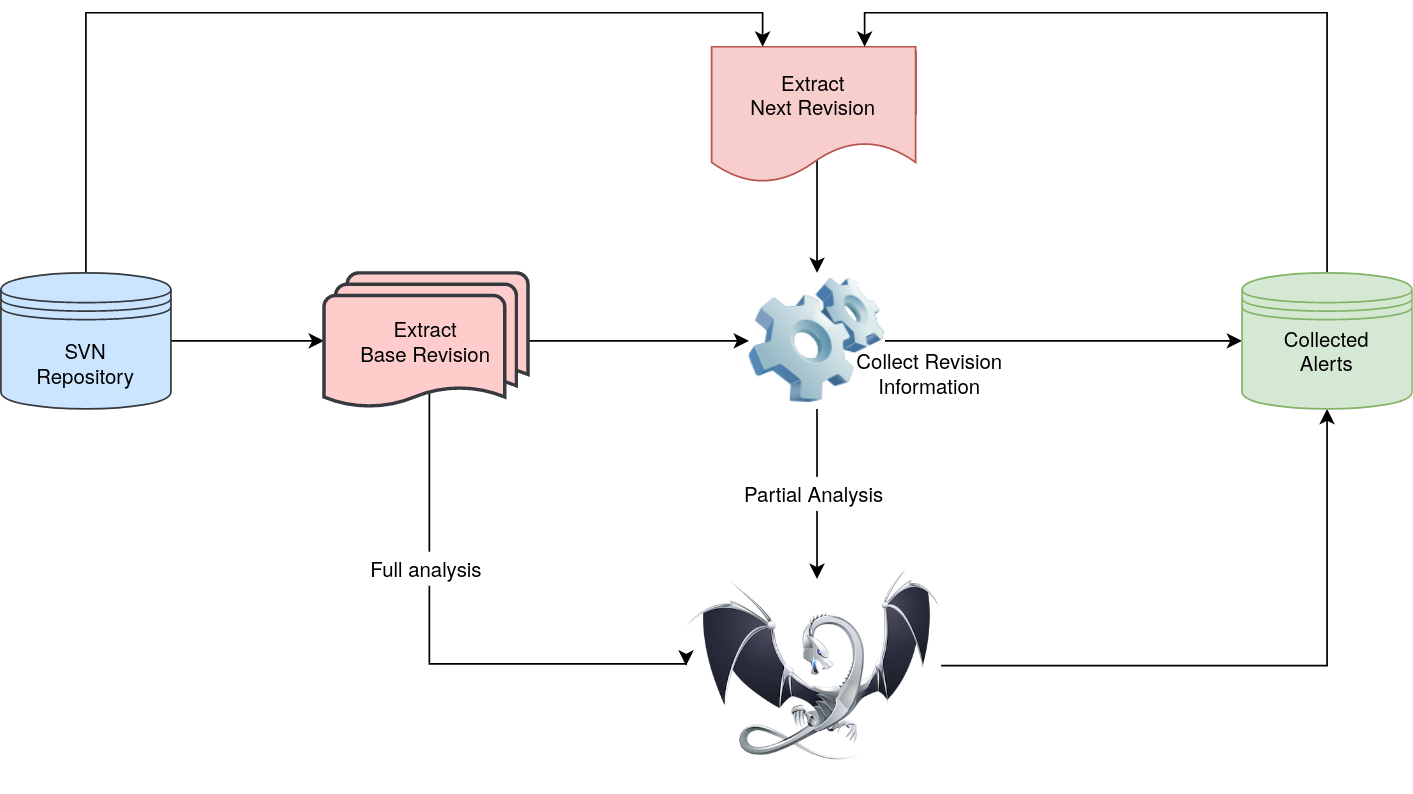
\includegraphics[scale=0.2]{./src/collect_info.png}
	\caption{Collecting alerts and other information}
\end{figure}

\subsubsection{Assumptions made for collected data}
Some algorithms use the notion of Actionable Alerts for processing the output of SA tools. Actionable Alerts (AA) are alerts that are deemed important by developers in the past (alerts that they acted on). In order to automatically label alerts as such (no existing information that can point to that), an important and risky assumption has to be made: alerts that disappear during code changes (revisions/commits) are considered as actionable, the rest is not. 

This assumptions, though necessary, is risky because not all alerts disappear as a result of direct and targeted change by developers. Their disappearance can be caused by other unknown factors (those related to deleted files are not taken into account). Data generated using this approach can contain a lot of false positives and potentially damage the performance of the used ML algorithms.

Another algorithm uses alerts pointing at past bugs as a way to prioritize future alerts. Also in this case an assumption is needed: the alerts that pointed to past bugs, were directly related to that bug. This may not always be true and can cause the aforementioned problems as a result.

The nature of automatic data extraction, without a reliable oracle pointing at the right decisions, leads to impure data and penalizes the efficiency of ML algorithms, but unfortunately it is an indispensable trade-off to be made.

\subsection{Data overview}

\textbf{TODO: Analyze of large portion of revisions and produce statistics}
\textbf{TODO: List which alert types were considered}
\textbf{TODO: Bug statistics for bug related lines}

There are X packages, Y files, Z lines of code.\\
Analyzed X revisions, from Y date to Z date.\\
There are these alerts per type.\\
Open/closed alerts statistics.\\
Alert distribution per type/package (graphs).\\


\subsection{Dealing with unbalanced and noisy data}

Our automatically collected data suffers from two main problems, heavy imbalance and noise. 

Kim et al. \cite{noise_defect} propose a method for dealing with noisy data in the context of defect prediction algorithms. They also provide guidelines for acceptable noise levels and study the impact of different amounts of noise on the prediction performance.
They found out that performance, in terms of f-measure, is affected more by the presence of false positives and that the tested algorithms were robust to the presence of false negatives. When noise levels reach 20-35\% of both FP and FN, the performance decreases significantly, especially on small datasets.
The proposed algorithm for cleaning noisy data by \cite{noise_defect}, calculates the ratio of the top \textit{N} most similar instances of each item that have a different class label. If that ratio exceeds a certain threshold, then that item is considered as noisy.

Batista et al. \cite{balancing_comparison}, perform a comparative evaluation of different dataset balancing techniques. They claim that imbalance alone is not the only reason for poor classifier results, but that it is also related to noisy/overlapping data. According to their experiments, over-sampling methods perform generally better and \textit{SMOTE} + Tomek/ENN provide good results for datasets with few positive examples.

Given the nature of our approach to detecting actionable alerts, it seems plausible that the amount of false positives will be non negligible, and thus there is a high risk that there will be a significant performance impact. Since, the number of examples of the positive class is also rather limited, there seems to be a necessity to apply a combination of balancing and cleaning to the dataset.

\textbf{TO DO: maybe insert before and after graph for data cleaning/balancing?}

\subsection{Feedback Rank and Z-Score}

% \textbf{TODO: maybe try a different correlation (author/alert type/?)}
% check vs naive bayes - trade off with speed

Feedback Rank (\cite{correlation_exploitation}) combined with Z-Score (\cite{z-ranking}) is a simple technique which ranks alerts on the probability of them being true/actionable. It consists of three basic features: package, file, function of the alert being analyzed (though may be extended as needed).
By constructing a Bayesian Network based on these three features and the history of the project (which alerts have been proven valuable) it produces a probability ranking about which alerts are most useful.

As explained on the literature review (\cref{literature}), Feedback Rank is based on the assumption that bugs and false positives are clustered by code locality. The alerts are divided into two major regions, one that contains mostly true positive, and one that contains mostly false positives. A Bayesian Network (BN) is used to calculate the probabilities of an alert or cluster of alerts belonging to a certain region.

\textbf{TODO: add graph of alert distribution for the project, similar to this paper}

The initial configuration of the network can learned from historical data (extracted as explained on \cref{data_collection}). Feedback Rank is supposed to be an online ranking system, if we inspect a report and know its value, the probabilities of the parents are re-calculated.

To construct the BN, the Pomegranate library was used (\cite{pomegranate}), trained with the extracted alert data from the version history.

\textbf{TO DO: used as static, explain zranking assumption, add prediction/train time}


\subsubsection{Z-Score}
To break ties when the probabilities provided by the BN are equal between alerts, the Z-Score metric is used based on the number of alerts on the same file. Z-Score is used in Z-Ranking (\cite{z-ranking}), which makes use of the observation that the most reliable error reports are those that generated few failed checks and many successful checks, since the actual amount of bugs in code is relatively small. 

The \textit{z-test} statistic, which measures how far an observed value is from the real population, in this case produces a large positive \textit{z-score} when there are few errors and many successes, and a large negative \textit{z-score} when there are few successes and many errors.

To make use of the Z-Score, an approximation is made. The granularity used for calculating the scores of alerts is based on file level (how many actionable/unactionable alerts of a certain type in a file), instead of the original granularity of the alert (for example an alert that only works on \textit{for loops}). This approximation is made because we do not know for each alert in which code construct it works on. Also, since it is only used as a tie-breaker, a high precision is not indispensable.

\subsection{Detecting Actionable Alerts via Machine Learning}
% classifiers used, how to train (grid search), overfitting, ways to measure

Different research papers have focused on automatically classifying alerts in true/false positives or actionable/unactionable, by constructing classifiers based on code or change metrics (\cite{actionable_sa}, \cite{model_building_actionable}).

Instead of focusing on classifying alerts as true or false positives, we focus on Actionable Alerts instead: alerts that are deemed important by the developers (not restricted to the type of alerts, but also to the context on which it manifests itself). The later is a less restrictive definition and makes it easier to collect data. Classifying alerts as true or false would necessitate an oracle telling which is which or a large and representative dataset generated manually. In addition, from a developer's perspective, AAs can be more useful. An alert can be true but might be considered not important by developers and thus be equally useless as a false one (low criticality, no impact on user side etc...).

Research is conducted by following the example of \cite{model_building_actionable}, since it contains an agglomeration of alert characteristics (AC) collected from other research papers.

The workflow, as explained in \cref{data_collection}, consists of iterating through the version history, collecting alerts characteristics and keeping track which alerts disappear (considered as actionable). ACs are then later used as features in ML algorithms with actionability being the target to predict.

The scikit-learn library was used to perform ML experiments (\cite{scikit-learn}).

\subsubsection{Alert Characteristics}

The collected ACs can be classified in five main categories: alert information, source code metrics, version history, churn metrics, and aggregate characteristics.

\paragraph{Alert information:} (a) package name (or folder), (b) file name, (c) file extension, (d) alert type, (e) alert category (security, core guidelines...), (f) method signature.

\paragraph{Source code metrics:} (a) number of statements, (b) number of methods, (c) number of classes, (d) cyclomatic complexity.

\paragraph{Version history:} (a) alert open revision, (b) developers who made changes from the open revision of an alert to revision under analysis, (c) file creation revision, (d) file deletion revision, (e) latest modification revision.

\paragraph{Churn metrics:} (a) added lines, (b) deleted lines, (c) growth (added-deleted), (d) total modified (added+deleted), (e) percent modified.

\paragraph{Aggregate characteristics:} (a) total alerts for revision, (b) total open alerts for revision, (c) alert lifetime, (d) file age, (e) alerts for artifact (method, file, package), (f) staleness (amount of time since last change of file, method, package).


\subsubsection{Pre-processing data}

***mostly categorical data -> tree based algorithms\\
\textbf{***do not use label encoding with nominal data (false order)}\\
\textbf{***try other encoding techniques}

\paragraph{Label encoding} Some algorithms need data in numerical form. Since most of the features are categorical data, we need a way to convert them to numerical. A simple approach was chosen, label encoding, which assigns an integer to each value of a category. Other approaches such as One-Hot encoding would increase the amount of data a lot (ex. consider one-hot encoding the file where an alert a method is from, which is a feature with high cardinality).

\paragraph{Imbalanced dataset} A quick look at the number of closed or not closed alerts shows that the dataset is heavily unbalanced. In order to train the ML algorithms we need first to balance the dataset. Two main techniques were tried: random undersampling and SMOTE (by using the library from \cite{imblearn}).\\

\textbf{TO DO:}\\
-cite paper where oversampling works better\\
-list other metrics\\
-explain balancing techniques?

\paragraph{Scaling} While for tree based algorithms scaling is not needed, for other algorithms like Logistic Regression, scaling the inputs can make a difference.

\paragraph{Missing values} In some ACs data may be missing, for example...

\paragraph{Feature selection} The features needed to train the models vary from project to project. Since collecting features that have little to no impact on algorithm performance is a waste of resources, techniques can be applied to select the most representative subset of features. Two main techniques were used: PCA and Recursive Feature Elimination.
\textbf{TODO: COMPARISON FULL FEATURES VS REDUCED}
% correlations?

\subsection{Bug related lines}

Another automatic way to determine which alerts are useful is to check if they pointed to lines that were changed during bug fixes. By doing so, we are regarding as valuable only those alerts that potentially signaled future bugs. The concept of bug related lines (BRL) is used in \cite{which_warnings} and \cite{automatic_training_set}.

BRLs are calculated as follows:
\begin{itemize}
    \item We start at a base revision and iterate backwards to a target revision. 
    \item If revision under analysis is a bug-fixing revision (contains a bug ID) collect changed/deleted code lines from the version history.
    \item If those collected lines were present in the code at least since the target revision, we consider them bug related lines.
    \item Continue iterating backwards, collecting BRLs. If previous lines that were considered BRL were changed before reaching the target revision, we remove them from the set. 
\end{itemize}

\begin{figure}[H]
    \centering
    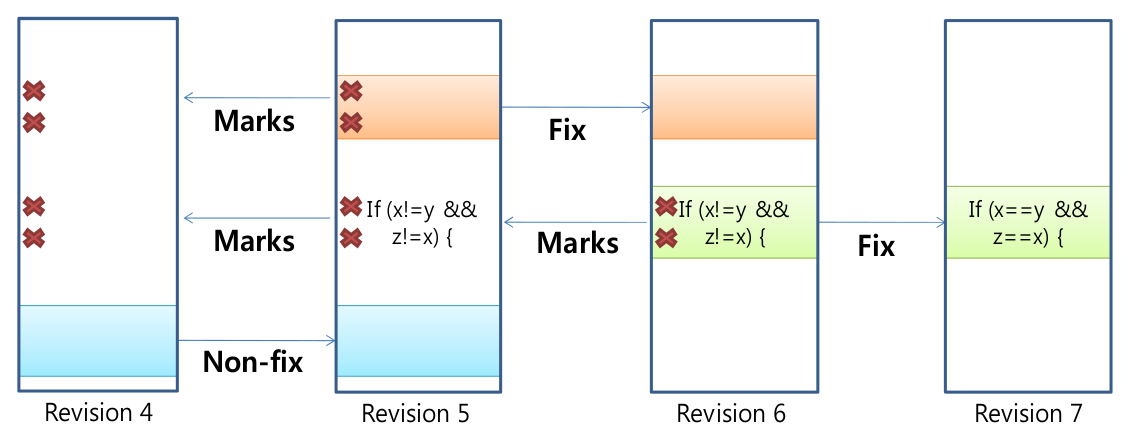
\includegraphics[scale=0.3]{./src/brl_example.png}
    \caption{Calculating BRLs (\cite{which_warnings})}
\end{figure}

% generic BRL vs project specific BRL

Since the amount of collected lines and warnings can be rather limited, we extend the definition to Bug Related Methods (BRM). Namely, we trace in which methods the BRL belong to and also consider alerts inside those methods as valuable. That allows to extend the dataset, but also potentially weakens the data by introducing more noise.

Given that the number of alerts collected this way, is a lot less than the total number of alerts, this method is more suited for ranking alert types rather than individual alerts (as used in \cite{which_warnings}).

\begin{figure}[ht]
	\centering
	\begin{minipage}{.5\linewidth}
		\begin{algorithm}[H]
			\SetAlgoLined
			\KwData{Collected bug-related alerts}
			\KwResult{Weighted alert types}
			$\alpha, \beta = x, y$\;
			$w_t = 0 \ for \ t \ in \ alertTypes$\;
			\For{alert in collectedAlerts}{
				$w_t = typeOf(alert)$\;
				\If{alert pointed to a BRL}{
					$w_t = w_t + \alpha$
				}
			
				\ElseIf{alert pointed to a BRM}{
					$w_t = w_t + \beta$
				}
			}
			\caption{Alert type priotitization algorithm}
		\end{algorithm}
	\end{minipage}
\end{figure}

\subsection{Bug prediction}

Following the example of \cite{static_profiling}, which aims to prioritize alerts based on the execution likelihood of the code pointed by the alert, we present a similar approach. Alerts pointing at potential bugs are the ones that can be considered the most important. The cost of detecting and fixing a bug is much lower if detected early in the development cycle. If we can predict which components will be likely to cause failures in the future, we can prioritize alerts that point to those components. 

The appropriate granularity to use for bug prediction is at method level. File level granularity is too broad since a lot of files contain many lines of code, which would result in prioritizing a lot of alerts, while anything lower than method level would be too hard to predict as bug prone.

We follow the example of the \cite{prediction_method} method. By using a combination of source code and change metrics and by exploiting the version history of the codebase, classifiers can be built that predict bug prone methods.

\begin{table}[H]
	\centering
	\begin{tabular}{@{}ll@{}}
		\textbf{Metric Name}          & \textbf{Description}                                                                                                                   \\ \midrule
		\textit{methodHistories}      & Number of times a method was changed                                                                                                   \\ \midrule
		\textit{authors}              & Number of distinct authors that changed a method                                                                                       \\ \midrule
		\textit{stmtAdded}            & Sum of all source code statements added to a method                                                                                    \\ \midrule
		\textit{maxStmtAdded}         & \begin{tabular}[c]{@{}l@{}}Maximum number of source code statements added \\ \\ to a method body for all method histories\end{tabular} \\ \midrule
		\textit{avgStmtAdded}         & \begin{tabular}[c]{@{}l@{}}Average number of source code statements added\\ to a method body per method history\end{tabular}           \\ \midrule
		\textit{stmtDeleted}          & \begin{tabular}[c]{@{}l@{}}Sum of all source code statements deleted from\\ a method body over all method histories\end{tabular}       \\ \midrule
		\textit{maxStmtDeleted}       & \begin{tabular}[c]{@{}l@{}}Maximum number of source code statements\\ deleted from a method body for all method histories\end{tabular} \\ \midrule
		\textit{avgStmtDeleted}       & \begin{tabular}[c]{@{}l@{}}Average number of source code statements\\ deleted from a method body per method history\end{tabular}       \\ \midrule
		\textit{churn}                & \begin{tabular}[c]{@{}l@{}}Sum of stmtAdded - stmtDeleted over all\\ method histories\end{tabular}                                     \\ \midrule
		\textit{maxChurn}             & Maximum churn for all method histories                                                                                                 \\ \midrule
		\textit{avgChurn}             & Average churn per method history                                                                                                       \\ \midrule
		\textit{decl}                 & \begin{tabular}[c]{@{}l@{}}Number of method declaration changes over all\\ method histories\end{tabular}                               \\ \midrule
		\textit{cond}                 & \begin{tabular}[c]{@{}l@{}}Number of condition expression changes in a\\ method body over all revisions\end{tabular}                   \\ \midrule
		\textit{elseAdded}            & \begin{tabular}[c]{@{}l@{}}Number of added else-parts in a method body\\ over all revisions\end{tabular}                               \\ \midrule
		\textit{elseDeleted}          & \begin{tabular}[c]{@{}l@{}}Number of deleted else-parts from a method\\ body over all revisions\end{tabular}                           \\ \midrule
		\textit{cyclomaticComplexity} & Current cyclomatic complexity of method                                                                                                \\ \midrule
		\textit{nestingDepth}         & Current nesting depth of method                                                                                                        \\ \midrule
		\textit{totalStatements}      & Current number of statements in method                                                                                                 \\ \midrule
		\textit{nrPaths}              & Current number of paths in method                                                                                                      \\ \midrule
		\textit{nrDeclarations}       & Current number of declarations in method                            \\\midrule 
	\end{tabular}
\end{table}

% rank alerts in problematic zones higher - combine with BRL?

\subsection{Combining the techniques}
% \subsection{Individual alert tuning}
% zranking cppcore guidelines
% COMBINE DIFFERENT TECHNIQUES FOR DIFFERENT ALERTS

\subsubsection{How to combine the strengths?}
% deep learning? make it flexible, learn with time\\
apply each technique to a subset of the warnings (which is more appropriate)

\subsubsection{Better results?}
Does it provide better results?


\subsection{Evaluation methods}

To evaluate and compare the approaches different techniques are used: 
\begin{itemize}
    \item \textbf{K-Fold Cross Validation}: where the data is randomly divided into folds and one of those is used for testing while the rest for training. It is often used in papers containing ML approaches to ranking alerts, though it has its drawbacks. As shown in \cite{performance_method_bug} and as can be seen on \cref{kfold_vs_release}, this approach uses dependent variables (most of the extracted features), that may not be available at prediction time in a real world scenario. That can lead to unreliable and excessively optimistic results.
    \item \textbf{Release/Revision based testing}: avoids the drawback of the previous method, by using a \textit{"horizontal"} train/test strategy. We fix a certain point in time (revision or release) which defines what the train set (before that point) and test set (after that point) will be. This trains the algorithms with more realistic data, but it also has its drawbacks. In a scenario where the dataset is imbalanced, a \textit{"horizontal"} 80/20\% split may leave us with very little data. Also, unlike in cross validation, we cannot train and test different models.
    \item \textbf{Alert ratio}: where we compare how much better is the ranking produced by a model with a random order of alerts. We calculate that by checking how many more alerts are better placed in the ranked version than the random one.
    \item \textbf{Average inspected false positives}: similar to the previous method where we compare the ranking produced by a model against a random one, but by calculating the average  number of times an unactionable alert has to be inspected before reaching an actionable one.
    \item \textbf{Fault detection rate curve}: the curve of a model is formed by the percentage of all actionable alerts found within the first \textit{X} alerts of the alert
    ranking algorithm.
    
    TO DO: see \cite{compare_framework} and apply only on top x\%? Fault detection rate curve?
    
    % \item Feedback-Rank paper has some approaches.
\end{itemize}

\begin{figure}[H]
    \centering
    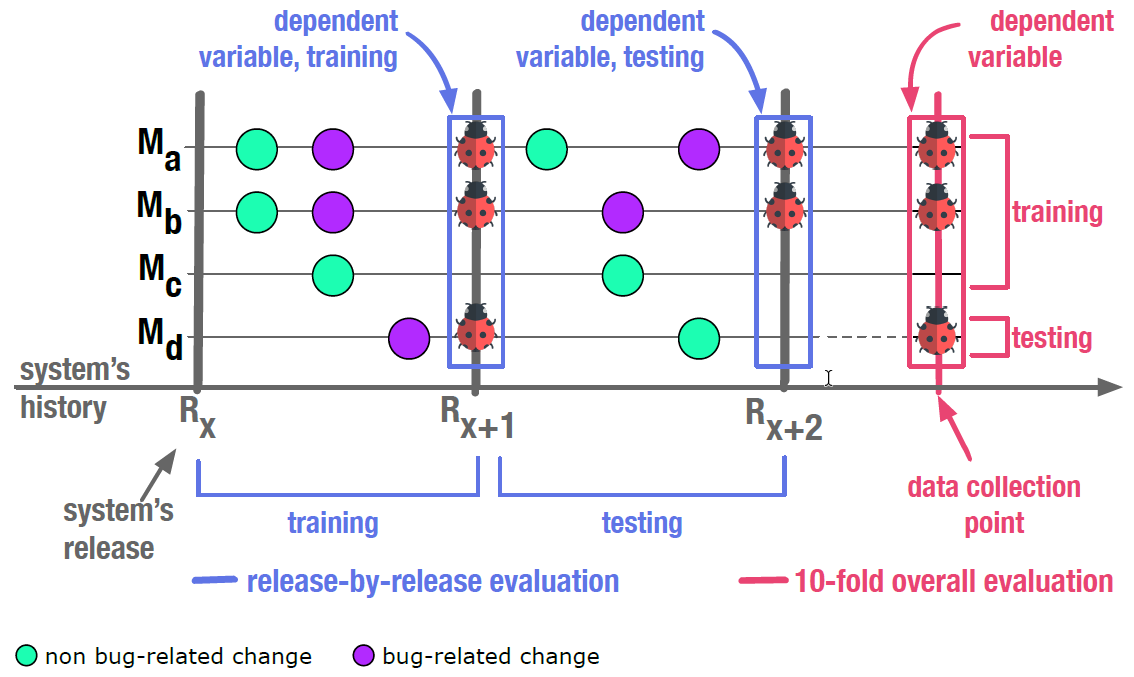
\includegraphics[scale=0.3]{./src/release_based_testing.png}
    \caption{Release-based vs K-Fold (\cite{performance_method_bug})}
    \label{kfold_vs_release}
\end{figure}

\subsubsection{Evaluation Metrics}

Along with the classic evaluation metrics like \textit{accuracy}, \textit{precision} and \textit{recall}, other metrics are used that are more appropriate for imbalanced data (\cite{comparison_metrics}, \cite{iba_metric}). 


\begin{gather*}
Sensitivity = \frac{TP}{TP + FN}\\
Specificity = \frac{TN}{FP + TN}\\
G-Mean = \sqrt{Sensitivity * Specificity}
\end{gather*} 
Sensitivity, or True Positive Rate is the percentage of positive examples which
are correctly classified.\\
Specificity, or True Negative Rate, is the percentage of negative examples which are correctly classified.\\
G-Mean is the geometric mean of the sensitivity and specificity.


\begin{gather*}
AUC = \frac{Sensitivity + Specificity}{2} \qquad (*approximation \ using \ trapezoid \ rule)
\end{gather*} 
The \textit{AUC} of a binary classifier is equivalent to the probability that the classifier will rank a randomly chosen positive instance higher than a randomly chosen negative instance.


\begin{gather*}
IBA_{\alpha} = (1 + \alpha * (Sensitivity - Specificity)) * Sensitivity * Specificity
\end{gather*} 
The \textit{Index of Balanced Accuracy} used for evaluating learning processes in two-class imbalanced domains. The
method combines an unbiased index of its overall accuracy and a measure about
how dominant is the class with the highest individual accuracy rate.


\subsubsection{Preparing the dataset}
Since the amount of actionable warnings is very low compared to the total amount of warnings, the dataset is balanced in two steps. First a subset of the packages and warnings is selected. By considering the ratio of actionable to the total amount of alerts, we can select the packages or types of warnings with the higher ratio (ex. the first 100).

After the first step, a test set is selected for evaluating the algorithms (equal to 20\% of the dataset).
That is especially needed to test the algorithms after the K-Fold evaluation.

The second step consists of balancing the amount of actionable and not actionable alerts, either by random subsampling or by artificially creating new samples (via SMOTE).


\textbf{TODO: EVALUATE OVERSAMPLING METHODS}

\textbf{TODO: EVALUATE ENCODING METHODS}

\subsection{Results of individual tools}

\subsubsection{Random test set}
\subsubsection{Release based testing}
\subsubsection{Alert ratio}
\subsubsection{Average false positives to inspect}


% results of each tool\\
% how to prepare a fair dataset:  normal vs release based\\
% personal feedback


% \section{Other approaches}

% \subsection{Other stuff}
% execution analysis?\\
% ir for bug messages

\section{Threats to Validity}
\henrique{In any empirical research, we must analysed and categorize the threats to validity of the experiments. The threats are classified into four cateegories: Construct Validity, Conclusion Validity, Internal Validity, and External Validity}



\section{Conclusions}
% You generally cover three things in the Conclusions section, and each of these usually merits a separate subsection:

% 1. Conclusions
% 2. Summary of Contributions
% 3. Future Research

% Conclusions are not a rambling summary of the thesis: they are short, concise statements of the inferences that you have made because of your work. It helps to organize these as short numbered paragraphs, ordered from most to least important. All conclusions should be directly related to the research question stated in Section 4. Examples:

% 1. The problem stated in Section 4 has been solved: as shown in Sections ? to ??, an algorithm capable of handling large-scale Zylon problems in reasonable time has been developed.
% 2. The principal mechanism needed in the improved Zylon algorithm is the Grooty mechanism.
% 3. Etc.

% The Summary of Contributions will be much sought and carefully read by the examiners. Here you list the contributions of new knowledge that your thesis makes. Of course, the thesis itself must substantiate any claims made here. There is often some overlap with the Conclusions, but that's okay. Concise numbered paragraphs are again best. Organize from most to least important. Examples:

% 1. Developed a much quicker algorithm for large-scale Zylon problems.
% 2. Demonstrated the first use of the Grooty mechanism for Zylon calculations.
% 3. Etc.

% The Future Research subsection is included so that researchers picking up this work in future have the benefit of the ideas that you generated while you were working on the project. Again, concise numbered paragraphs are usually best. 

\textbf{TO DO: FEASIBILITY STUDY BECAUSE OF LIMITED AMOUNT OF DATA}

\subsection{Conclusions}
-got these results, because...\\
-importance on preprocessing\\
-initial results may be slightly better that normal, but the nature of data collection is limiting, need to be used in continuance\\ 

% \begin{itemize}
%     \item Ranking can be useful but only with enough data
%     \item X method performs better / is more useful than Y
%     \item Combining techniques give these different results
%     \item Context of industrial code
% \end{itemize}


\subsection{Summary of Contributions}
 
 This thesis provides the following contributions:
 \begin{itemize}
     \item Building a workflow to extract information by making use of the Clang toolset and version history (SVN).
     \item Evaluating SA ranking techniques on an industrial codebase.
     \item Evaluating preprocessing techniques to deal with highly imbalanced and noisy data.
     \item Detailed report of ML workflow (not a lot of information on most papers)
     \item Comparing different approaches on a common codebase.
     \item Exploring the utility of combining different methods.
 \end{itemize}
 
% -building workflow to extract information\\
% -evaluation on industrial code\\
% -comparison of utility between tools\\
% -evaluation of an ensemble technique

\subsection{Future Research}

%Analyze the parts where the prediction fails?

Future research can be focused on different aspects, the most important being reliable data collection. A classifier is as good as the data it was trained on, so new ways to collect actionable alerts in a more precise way are crucial to achieving better performance. Information Retrieval or Natural Language Processing techniques can be applied for example on bug messages/descriptions to have a clearer connection between a bug and an alert (did the alert really predict the bug?).

Given also the limited amount of data, new or improved approaches that can generalize easily are needed. In that regard, research can focus on the type of features extracted from the code or version history that are discriminative enough to make correct classification even with limited data. FEATURE ENGINEERING, high cardinality, categorical data

Furthermore, given the diverse nature of alerts current tools have, from finding bugprone construct, stylistic alerts, library-oriented alerts, to security or performace-oriented checks, different methods can be tailored that maximise performance within these subsets of alerts. For example, a simple method like Z-Ranking (\cite{z-ranking}) can be more suited to predict stylistic alerts than others.

In addition, a way to continuously improve the ML algorithms needs to be put in place. Even though the initial performance may not be spectacular, if new resolved alerts are tracked consistently, performance will also rise accordingly. A rather naive implementation is to give warnings an identifier and include them in the commit messages if they were useful.

% -data collection assumptions, make it more reliable?\\
% -better track resolved alerts (google tricorder example)
% -information retrieval on bug messages
% TO DO


\nocite{*}
\bibliographystyle{unsrt}
\bibliography{references}

\end{document}